\documentclass[
	letterpaper
]{article}

\usepackage{listings}
\lstset{language=Python,
    basicstyle=\ttfamily\small,
    stringstyle=\color{red},
    otherkeywords={0,1,2,3,4,5,6,7,8,9},
    morekeywords={TRUE,FALSE},
    deletekeywords={_data,data,frame,length,character},
    keywordstyle=\color{blue},
    commentstyle=\color{gray},
    showstringspaces=false,
}
\usepackage{array}
\usepackage{amsmath}
\usepackage{graphicx}
\usepackage{xcolor}
\usepackage{float}
\usepackage{hyperref}
\usepackage{caption}
\usepackage{subcaption}
\usepackage{xcolor}
\hypersetup{
    colorlinks,
    linkcolor={red!50!black},
    citecolor={blue!50!black},
    urlcolor={blue!80!black}
}


\title{Linear Regression built from scratch}
\date{}

\begin{document}
\maketitle
Linear regression is a supervised learning algorithm that has a deep root from statistics. 
It is one of the machine learning algorithms that look quite simple yet can be surprisingly useful.
In this article, we present the basics of a linear regression learner and build one from scratch using Python.

\section{What is regression?}
Regression is one type of supervised machine learning.

Well that does not appear to help a lot.
Let's start with one real-life example instead.
When we build a bookshelf, we have to choose which plywood to use.
From common sense, we know if our bookshelf is wide, we need thicker or stronger plywood, otherwise the bookshelf would bow or sag because of the weight of books.
In contrast, if our bookshelf is narrow, perhaps thinner or weaker plywood would be fine.
In that case, using thicker or stronger plywood would add unnecessary cost and thus is not an optimal choice.

Here we have two groups of data: ``plywood'' and ``width of bookshelf''.
Our task is to answer this question: given our desired width of bookshelf, which plywood should we use?
If we call ``width of bookshelf'' as $x$ and ``plywood'' as $y$, then our task is ``given $x$, what is $y$?''

How do we answer this question? 

Admittedly there are many ways, but probably the go-to method for most people is simply looking around existing bookshelves.
We just look around, find existing bookshelves, gather their width and which plywood did they use, and then determine the plywood for our new bookshelves.
The underlying rationale is that we assume our new bookshelf is similar in nature to these existing ones. 
If the new bookshelf has similar width as some of the existing ones, maybe we can just go ahead and use a similar type or thickness of plywood as those ones.

In other words, to answer the question ``given $x$, what is $y$'', we just gather a bunch of existing $x$ and $y$.
We try to ``learn'' something from these existing $x$ and $y$.
Based on what we learned, we then make an educated guess of $y$ for our new $x$.
What we described here is a brief picture of supervised learning, in which the existing $x$ and $y$ are called \textit{training} data.
That is part of the story where the word $machine learning$ comes from, in which \textit{machine (computer)} is doing the \textit{learning} instead of us.

In the world of supervised learning, if $y$ is regarded to a label or a type, such as ``pine plywood'', ``cedar plywood'', ``redwood plywood'', and so on, then this problem is called ``classification''.
In contrast, if $y$ is regarded to a continuous number, such as the thickness of a wood piece like ``0.32 inch'', ``0.44 inch'', ``0.58 inch'', and so on, then this problem is called ``regression'', which is the topic of our discussion today.

We admit this is not a great regression example since dimensions in traditional woodworking are usually limited to multiples of 1/8 inch
Let's assume we have a high-tech workshop using CNC machines to do woodworking and we can achieve any random dimension like 0.572 inch, then this is truly a regression problem.

\section{Math expression of a linear regression}
A regression problem, like we said above, is to answer ``given $x$, what is $y$'' by looking at some existing pairs of $x$ and $y$.
In this setting, $x$ is usually called \textit{attribute} or \textit{feature}, while $y$ is usually called \textit{response} or \textit{outcome}.

Assuming we have $n$ existing pairs of $x$ and $y$, which we can written as 
\begin{equation}
X = \begin{bmatrix}
x_1 & x_2 & ... & x_n
\end{bmatrix}
\end{equation}
\begin{equation}
Y = \begin{bmatrix}
y_1 & y_2 & ... & y_n
\end{bmatrix}
\end{equation}

The task of regression is to find the relation from $x$ to $y$.
In machine learning, sometimes people call this as a \textit{function approximation}, emphasizing we are trying to approximate a function whose input is $x$ and output is $y$.
The function from $x$ to $y$ can be any type, but in linear regression, as the name implies, we assume this function is linear, which means $Y$ is approximately linear to $X$.
\begin{equation}
y \approx wx+b
\end{equation}

In this equation, $w$ is usually called \textit{coefficient} in statistics and \textit{weight} in machine learning, while $b$ is usually called \textit{intercept} in in statistics and \textit{bias} in machine learning.
The predicted or modeled outcome $wx+b$ is often denoted as $\hat y$.
\begin{equation}
\hat y = wx+b
\end{equation}

In the simplest case, when $X$ only has one attribute, like in our example, ``the width of bookshelf'', then $w$ is one single scalar.
This is often called \textit{simple linear regression (SLR)} in statistics.
\begin{equation}
\begin{bmatrix}\hat y_1 \\ \hat y_2 \\ ... \\ \hat y_n\end{bmatrix}
 = w\begin{bmatrix} x_1 \\  x_2 \\ ... \\ x_n\end{bmatrix}+b
\end{equation}

For most of the cases, $X$ often has more than one attribute. 
In our bookshelf example, maybe not only the width but also the height affects the choice of plywood.
For a lot of real-world problems, we have dozens or even hundreds of attributes and we might not know which attributes actually affect the outcome.
In these cases, $X$ is no longer a vector but a matrix, with rows representing different data \textit{points} or \textit{instances} and columns representing different data attributes or features.
This is often called \textit{multiple linear regression (MLR)} in statistics.
\begin{equation}
X =
\begin{bmatrix}
x_{1, 1} & x_{1, 2} & ... & x_{1, k} \\
x_{2, 1} & x_{2, 2} & ... & x_{2, k} \\
... & ... & ... & ... \\
x_{n, 1} & x_{n, 2} & ... & x_{n, k} \\
\end{bmatrix}
\end{equation}

In this $X$ matrix, $x_{i, j}$ represents the $j$th \textit{attribute} of the $i$th data \textit{instance}.
For example, $x_{1, 1}$ represents the width (1st attribute) of the 1st bookshelf (1st instance) and $x_{1, 2}$ represents the height (2nd attribute) of the 1st bookshelf (1st instance), while $x_{2, 1}$ represents width of the 2nd bookshelf and $x_{2, 2}$ represents the height of the 2nd bookshelf.

Accordingly, $w$ is no longer a scalar but a vector with a length of $k$, where $k$ is the number of attributes per instance.
\begin{equation}
\begin{bmatrix}\hat y_1 \\ \hat y_2 \\ ... \\ \hat y_n\end{bmatrix}
 = \begin{bmatrix}
x_{1, 1} & x_{1, 2} & ... & x_{1, k} \\
x_{2, 1} & x_{2, 2} & ... & x_{2, k} \\
... & ... & ... & ... \\
x_{n, 1} & x_{n, 2} & ... & x_{n, k} \\
\end{bmatrix}
\begin{bmatrix} w_1 \\  w_2 \\ ... \\ w_k\end{bmatrix}
+b
\end{equation}

For simplicity, we can also incorporate bias $b$ into vector $w$ by adding a column of 1 as the first column of $X$ and replacing $b$ with $w_0$.
\begin{equation}
\begin{bmatrix}\hat y_1 \\ \hat y_2 \\ ... \\ \hat y_n\end{bmatrix}
 = \begin{bmatrix}
1 & x_{1, 1} & x_{1, 2} & ... & x_{1, k} \\
1 & x_{2, 1} & x_{2, 2} & ... & x_{2, k} \\
... & ... & ... & ... & ... \\
1 & x_{n, 1} & x_{n, 2} & ... & x_{n, k} \\
\end{bmatrix}
\begin{bmatrix} w_0 \\ w_1 \\  w_2 \\ ... \\ w_k\end{bmatrix}
\end{equation}

This equation can then be written as matrix forms.
\begin{equation}
\hat Y= X w
\end{equation}

Now we have a math representation of the linear regression problem.
The true outcome is $Y = [y_1, y_2, ..., y_n]$ and the predicted outcome is $\hat Y = [ \hat y_1, \hat y_2, ..., \hat y_n]$.
Our task is then to finding the proper $w = [w_0, w_1, w_2, ..., w_k]$ so that $\hat Y$ is as close to $Y$ as possible.

\section{How far away is $\hat Y$ from $Y$?}
To achieve our task, the first thing we need to do is to define what do we mean by ``close''.
In other words, we need some quantitative measure to represent how far away is $\hat Y$ from $Y$.

To define this quantitative measure, let's use three different data sets plotted in Figure~\ref{fig:raw-data} as examples.
For simplicity, these data sets have the same $x$ with only one data attribute.
The horizontal axis plots $x$ and the vertical axis plots $y$.
\begin{figure}[htbp]
	\centering
	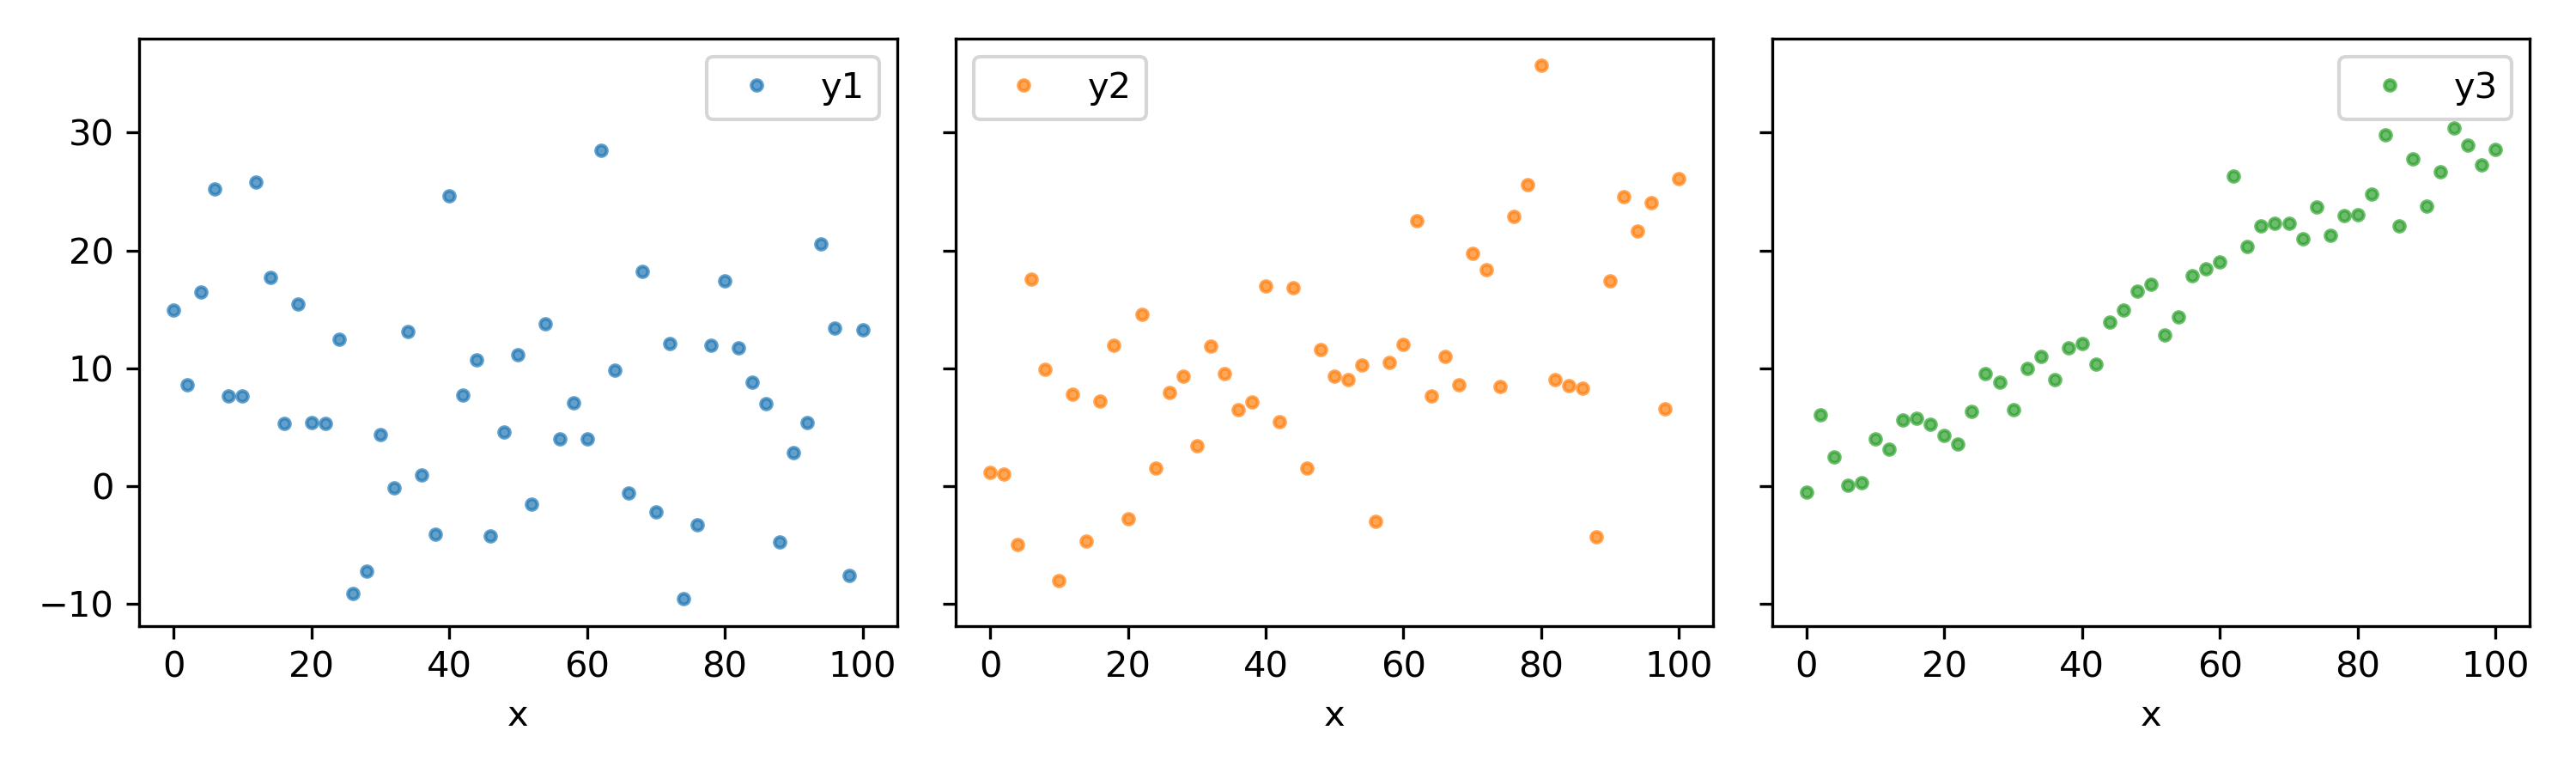
\includegraphics[width=0.98\textwidth]{figures/comparison-raw-data.png}
	\caption{$y$: true outcome}
	\label{fig:raw-data}
\end{figure}

First we ask this question: what is the worst prediction $\hat Y$ a reasonable person can make?

Admittedly, we can make a lot of arbitrarily bad predictions of $\hat Y$ that is absurdly not close to $Y$ at all.
However, as \textit{reasonable} people,  we can probably all agree that there is a baseline for $\hat Y$ which is $\bar y$, the mean value of $Y$.
In our bookshelf example, this means we will just use the average plywood thickness of existing bookshelves for any new bookshelf regardless of the width.
This choice might be wrong, but the point is that it is not absurdly wrong.
Usually, we can use this ``wrong'' answer as a baseline for further improvement.

In math expression, predicting everything as the mean of $Y$ is basically let $w_0$ be the average of $Y$ and let all other $w_j$ be 0.
\begin{equation}
\begin{bmatrix}\hat y_1 \\ \hat y_2 \\ ... \\ \hat y_n\end{bmatrix}
 = \begin{bmatrix}
1 & x_{1, 1} & x_{1, 2} & ... & x_{1, k} \\
1 & x_{2, 1} & x_{2, 2} & ... & x_{2, k} \\
... & ... & ... & ... & ... \\
1 & x_{n, 1} & x_{n, 2} & ... & x_{n, k} \\
\end{bmatrix}
\begin{bmatrix} \bar y \\ 0 \\  0 \\ ... \\ 0\end{bmatrix}
=
\begin{bmatrix} \bar y \\ \bar y \\ \bar y \\ ... \\ \bar y\end{bmatrix}
\end{equation}

In this case, our true outcome is $Y = [y_1, y_2, ..., y_n]$ and our predicted outcome is $\hat Y = [\bar y, \bar y, ..., \bar y]$.
In Figure~\ref{fig:sst}, the ``distance'' between these two is visualized as vertical lines connecting the corresponding $y_i$ and $\bar y$.
\begin{figure}[htbp]
	\centering
	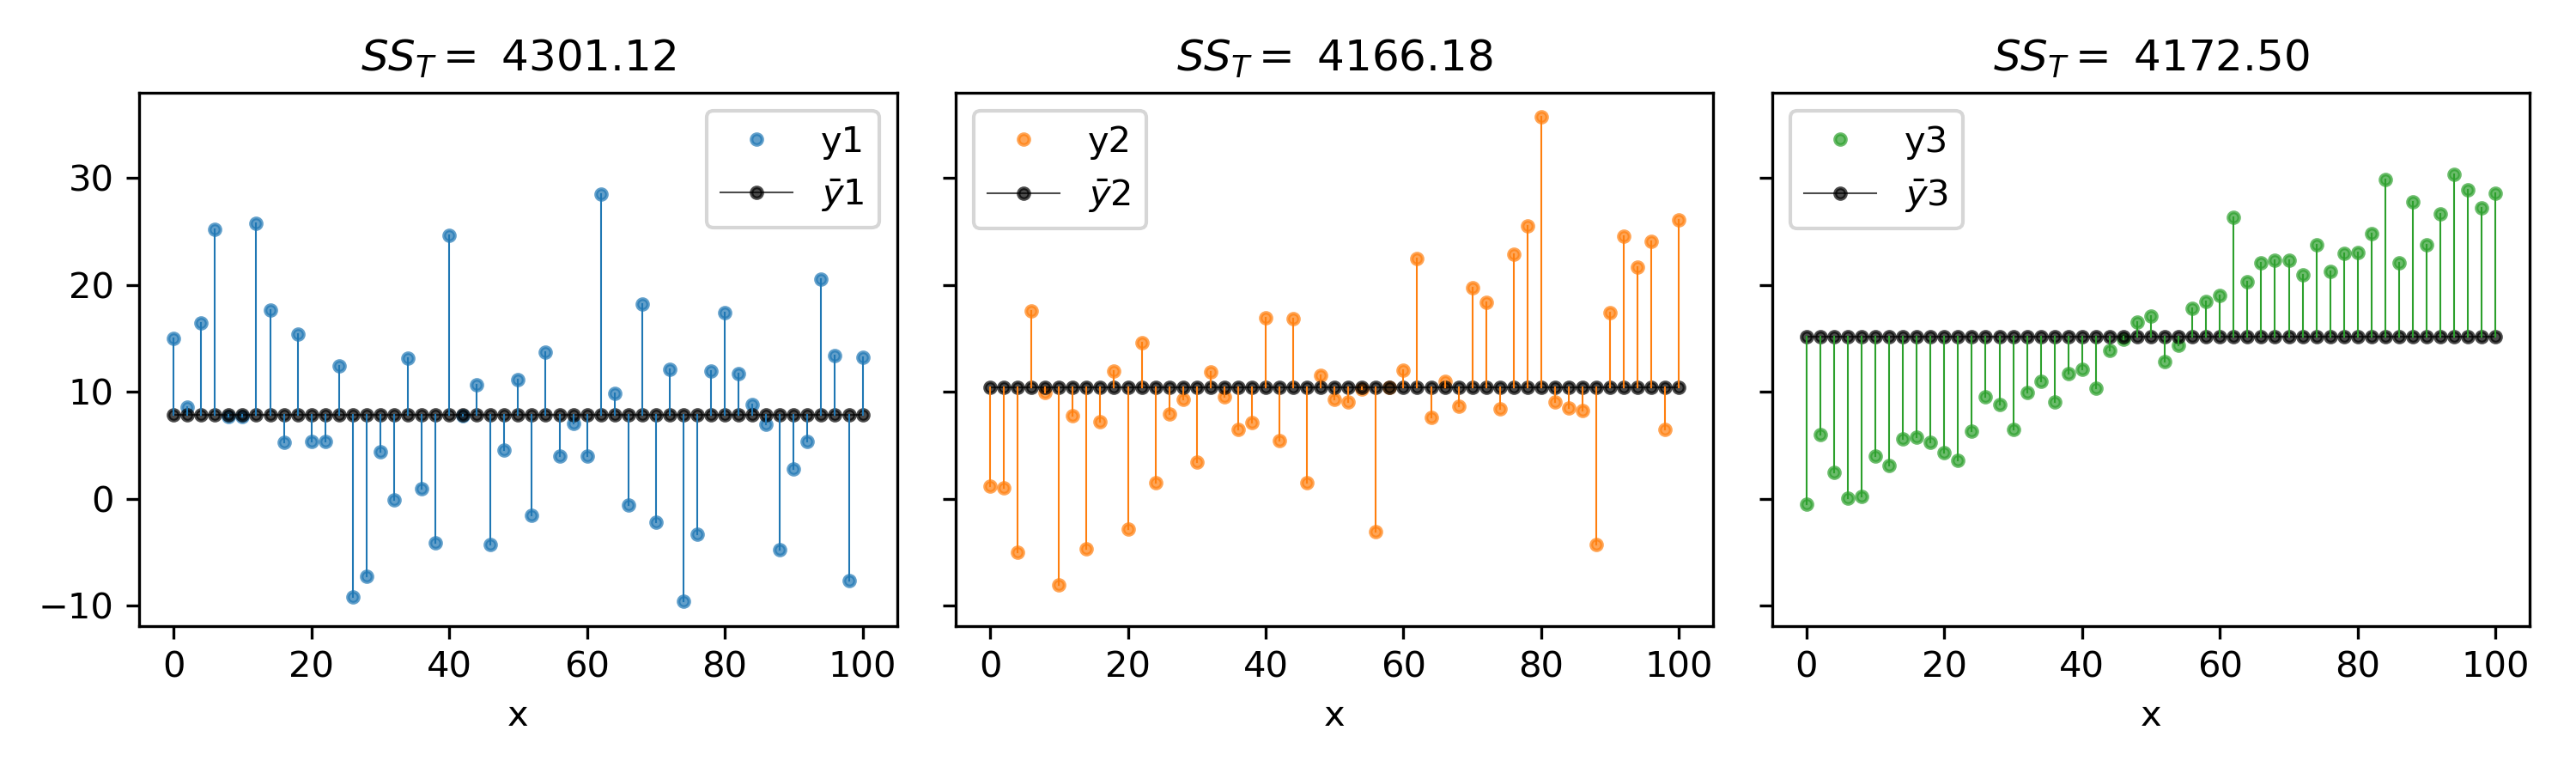
\includegraphics[width=0.98\textwidth]{figures/comparison-sst.png}
	\caption{$SS_T$: distance between $y$ and $\bar y$}
	\label{fig:sst}
\end{figure}

This distance can be defined quantitatively as the sum of square of the length of these vertical lines and is denoted as $SS_T$, which stands for \textit{total sum of squares}.
In some way, we can think of $SS_T$ as a baseline of our model.
A reasonable model should be at least works better than this.
In our example, all three data sets happen to have similar $SS_T$ of around 4150 to 4300.
\begin{equation}
SS_T = \sum_{i = 1}^n (y_i - \bar y) ^2 
\end{equation}

In our model, we have $[w_0, w_1, w_2, ..., w_k]$ which are different from $[\bar y, 0, 0, ..., 0]$ and we somehow believe our choice is better.
For now, let's assume we somehow get these $w_i$ magically and the predicted $\hat y$ are plotted in Figure~\ref{fig:yhat}.
\begin{figure}[htbp]
	\centering
	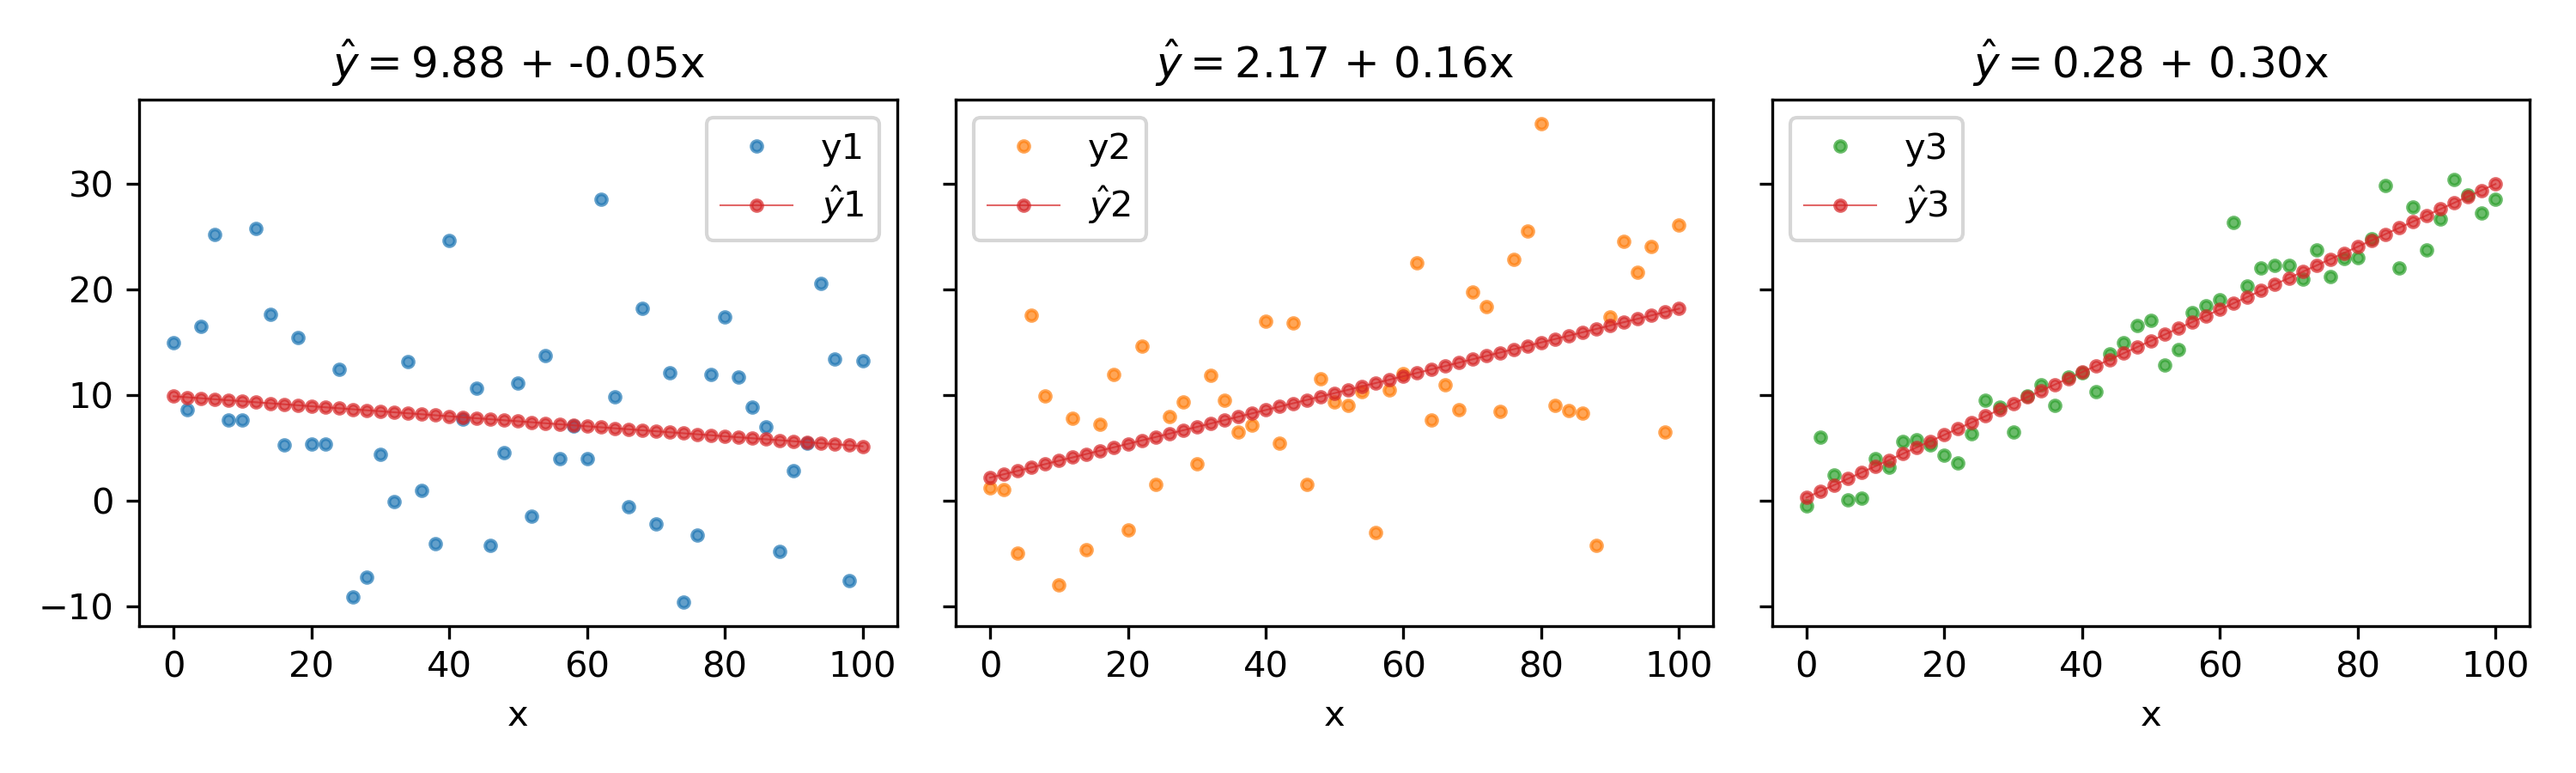
\includegraphics[width=0.98\textwidth]{figures/comparison-yhat.png}
	\caption{$\hat y$: predicted outcome from linear regression}
	\label{fig:yhat}
\end{figure}

Here comes our second question: how much better is our model compared to baseline?
Our model predicts the outcome as $\hat Y = [\hat y_1, \hat y_2, ..., \hat y_n]$ instead of $[\bar y, \bar y, ..., \bar y]$.
The ``distance'' between our model and the baseline is $SS_R$, which stands for \textit{regression sum of squares} (also called \textit{explained sum of squares}).
\begin{equation}
SS_R= \sum_{i = 1}^n (\hat y_i - \bar y) ^2 
\end{equation}

Figure~\ref{fig:ssr} visualizes the concept of $SS_R$, which is the sum of squares of the length of vertical lines.
We can think of $SS_R$ as how much better our model is compared with the baseline.
In other words, $SS_R$ tells us how helpful our model is.
For example, for the leftmost data set, $SS_R$ is 105 and $\hat y$ is not significantly different from $\bar y$.
This tells us this model is not very helpful as there is no significant difference between using $\hat y$ and simply using $\bar y$.
In contrast, for the rightmost data set, $SS_R$ is 3900 which tells us that this model is pretty useful as using $\hat y$ is significantly different (hopefully better) than simply using $\bar y$.
\begin{figure}[htbp]
	\centering
	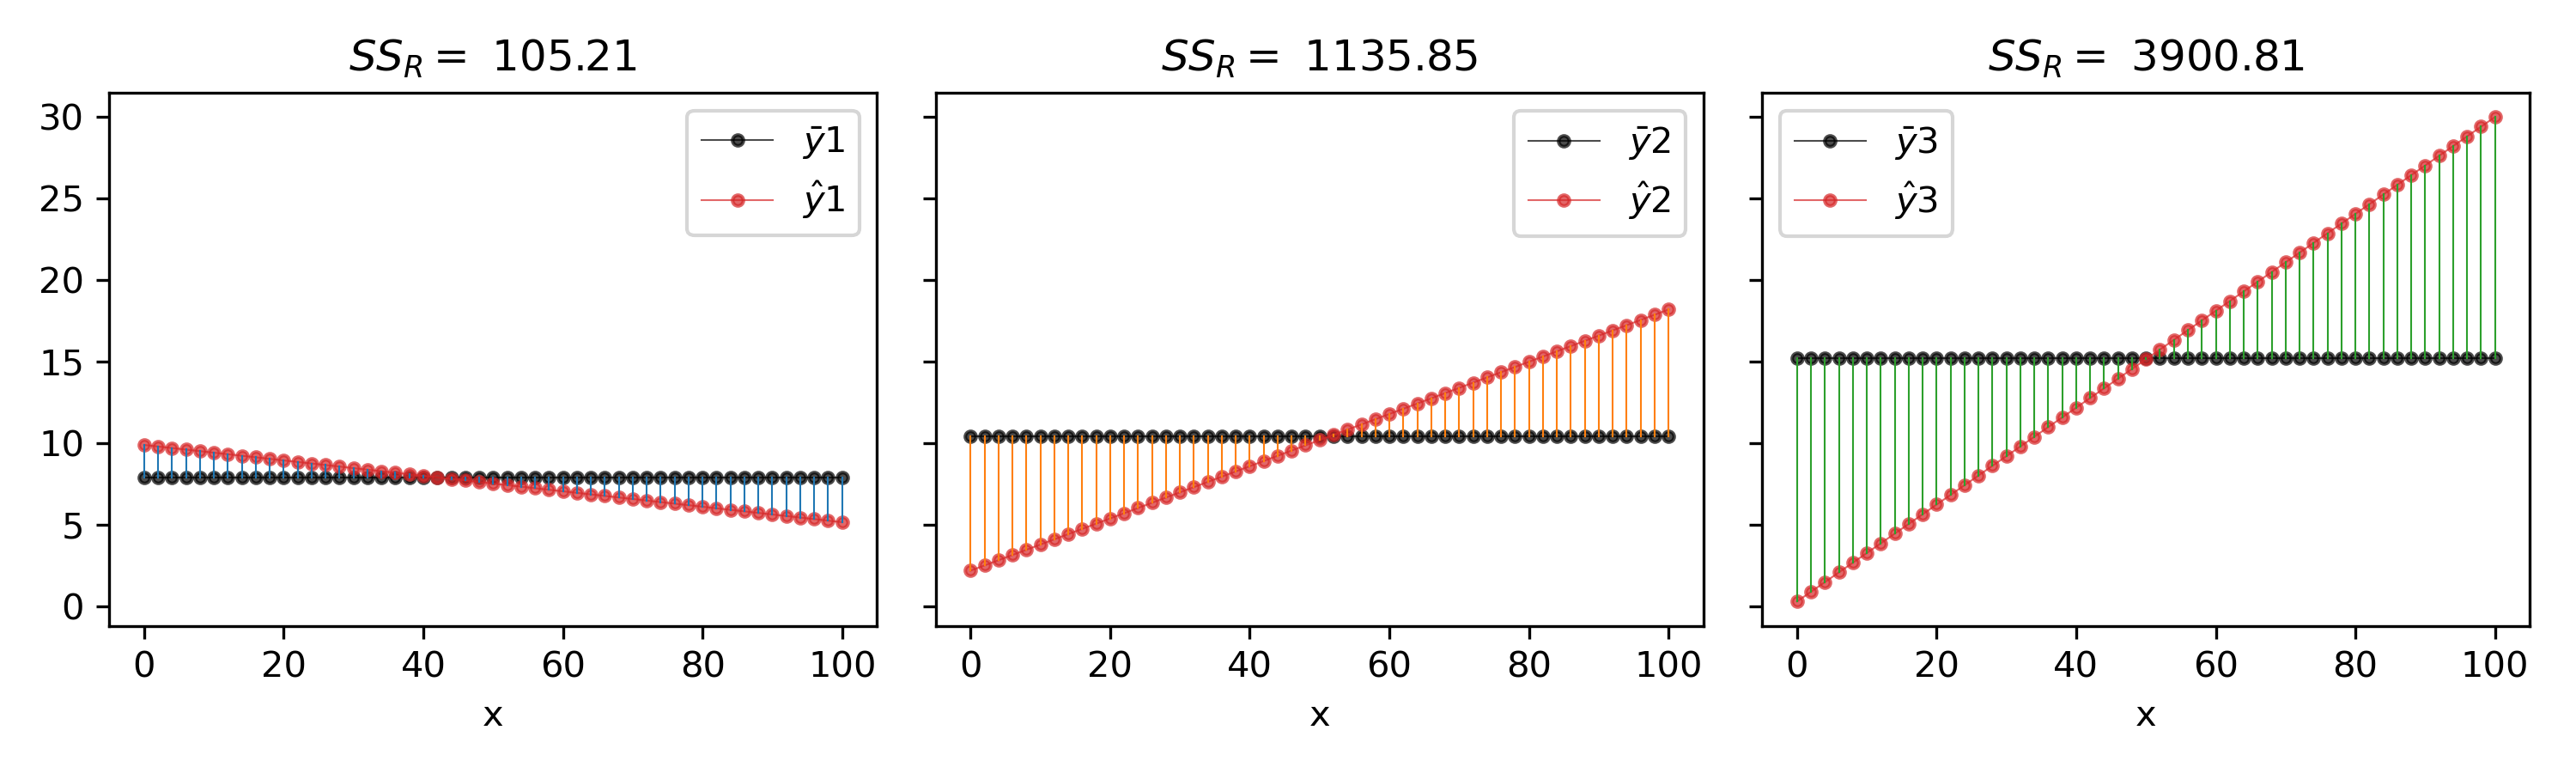
\includegraphics[width=0.98\textwidth]{figures/comparison-ssr.png}
	\caption{$SS_R$: distance between $\hat y$ and $\bar y$}
	\label{fig:ssr}
\end{figure}

Nevertheless, no matter how much better our model is, we probably will not achieve perfection. 
Our third question is how far away is our model from absolutely perfection?

Our model predicts the outcome as $[\hat y_1, \hat y_2, ..., \hat y_n]$ while the prefect answer is the true outcome $[y_1, y_2, ..., y_n]$.
The distance from our model to absolute perfectness is $SS_E$, which stands for \textit{error sum of squares}, (also called \textit{residual sum of squares}). 
\begin{equation}
SS_E = \sum_{i = 1}^n (y_i - \hat y_i) ^2 
\end{equation}

Figure~\ref{fig:sse} visualizes the concept of $SS_E$, which is the sum of squares of the length of vertical lines.
The smaller $SS_E$ is, the less ``error'', the closer our model is to perfection.
For example, $SS_E$ of the rightmost case is 235, which is the smallest among the three sets.
Correspondingly, $\hat y$ of the rightmost case is the  closest to its $y$ visually.
\begin{figure}[htbp]
	\centering
	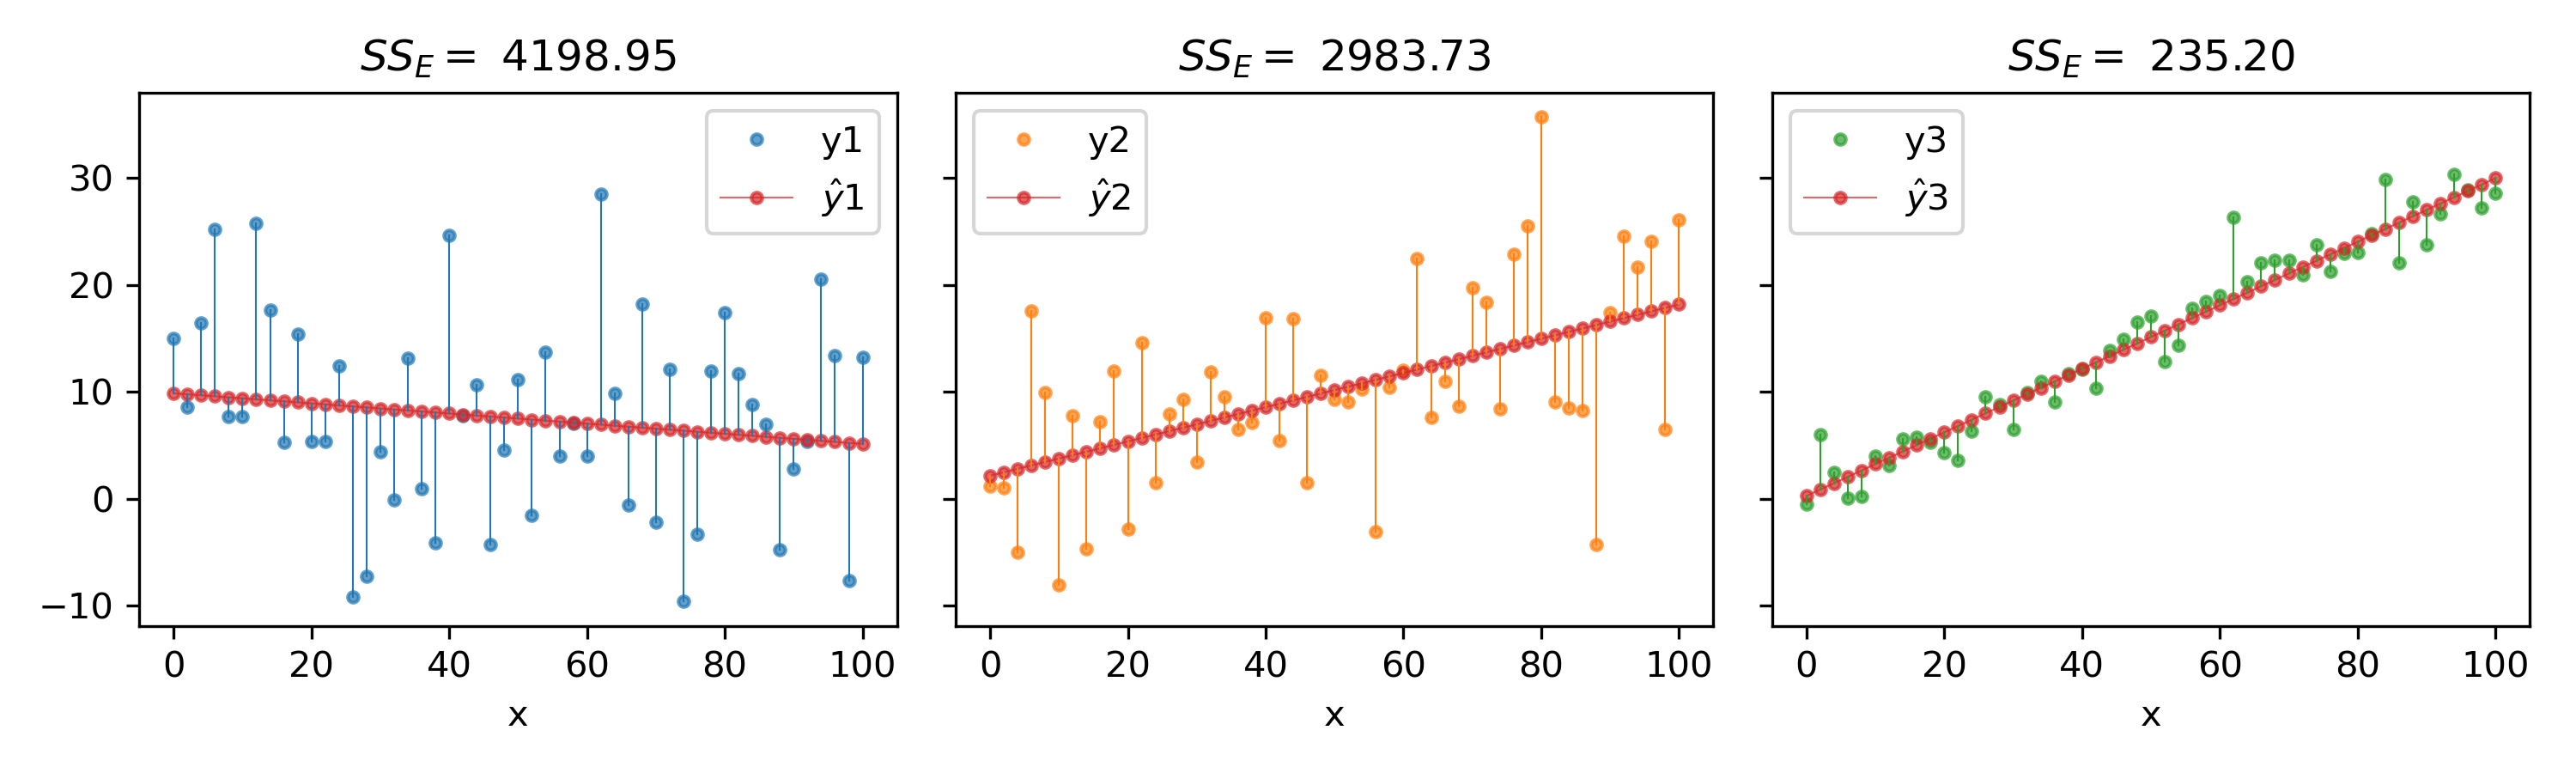
\includegraphics[width=0.98\textwidth]{figures/comparison-sse.png}
	\caption{$SS_E$: distance between $y$ and $\hat y$}
	\label{fig:sse}
\end{figure}

For these three example data sets, we can list the sum of squares in the following table:
\begin{table}[htbp]
	\small 
	\centering 
		\caption{Sum of squares of the three example data sets}
		\label{table:ss}
	\begin{tabular}{l | r r r}
$SS_T$										&		4301.12	&		4166.18		&	  4172.50\\
$SS_R$										&   105.21	&		1135.85		&  3900.81\\
$SS_E$										&		4198.95	&		2983.73		&  235.20\\
$SS_T - SS_E - SS_R$		&		-3.04	& 	46.60		&  36.49\\
$R^2 = 1-\frac{SS_E}{SS_T}$			&		2.4\%	&		28.4\%		&  94.4\%\\
	\end{tabular}
 \end{table}

For most of linear regression, in theory, it can be approved that 
\begin{equation}
SS_T = SS_R + SS_E
\end{equation}
In some sense, $SS_T$ is the distance from baseline to perfection, $SS_R$ is the distance from the baseline to our model, and $SS_E$ is the distance from our model to perfection.
A variable called R-Squared ($R^2$) is then defined as 
\begin{equation}
R^2 = 1 - \frac{SS_E}{SS_T} = \frac{SS_R}{SS_T}
\end{equation}

R-Squared is bounded between 0 and 1. The closer to 0, the closer our model is to baseline; the closer to 1, the closer our model is to perfectness.
For our example, as listed in the table, R-Squared is 2.4\%, 28.4\%, and 94.4\% respectively.
\begin{figure}[htbp]
	\centering
	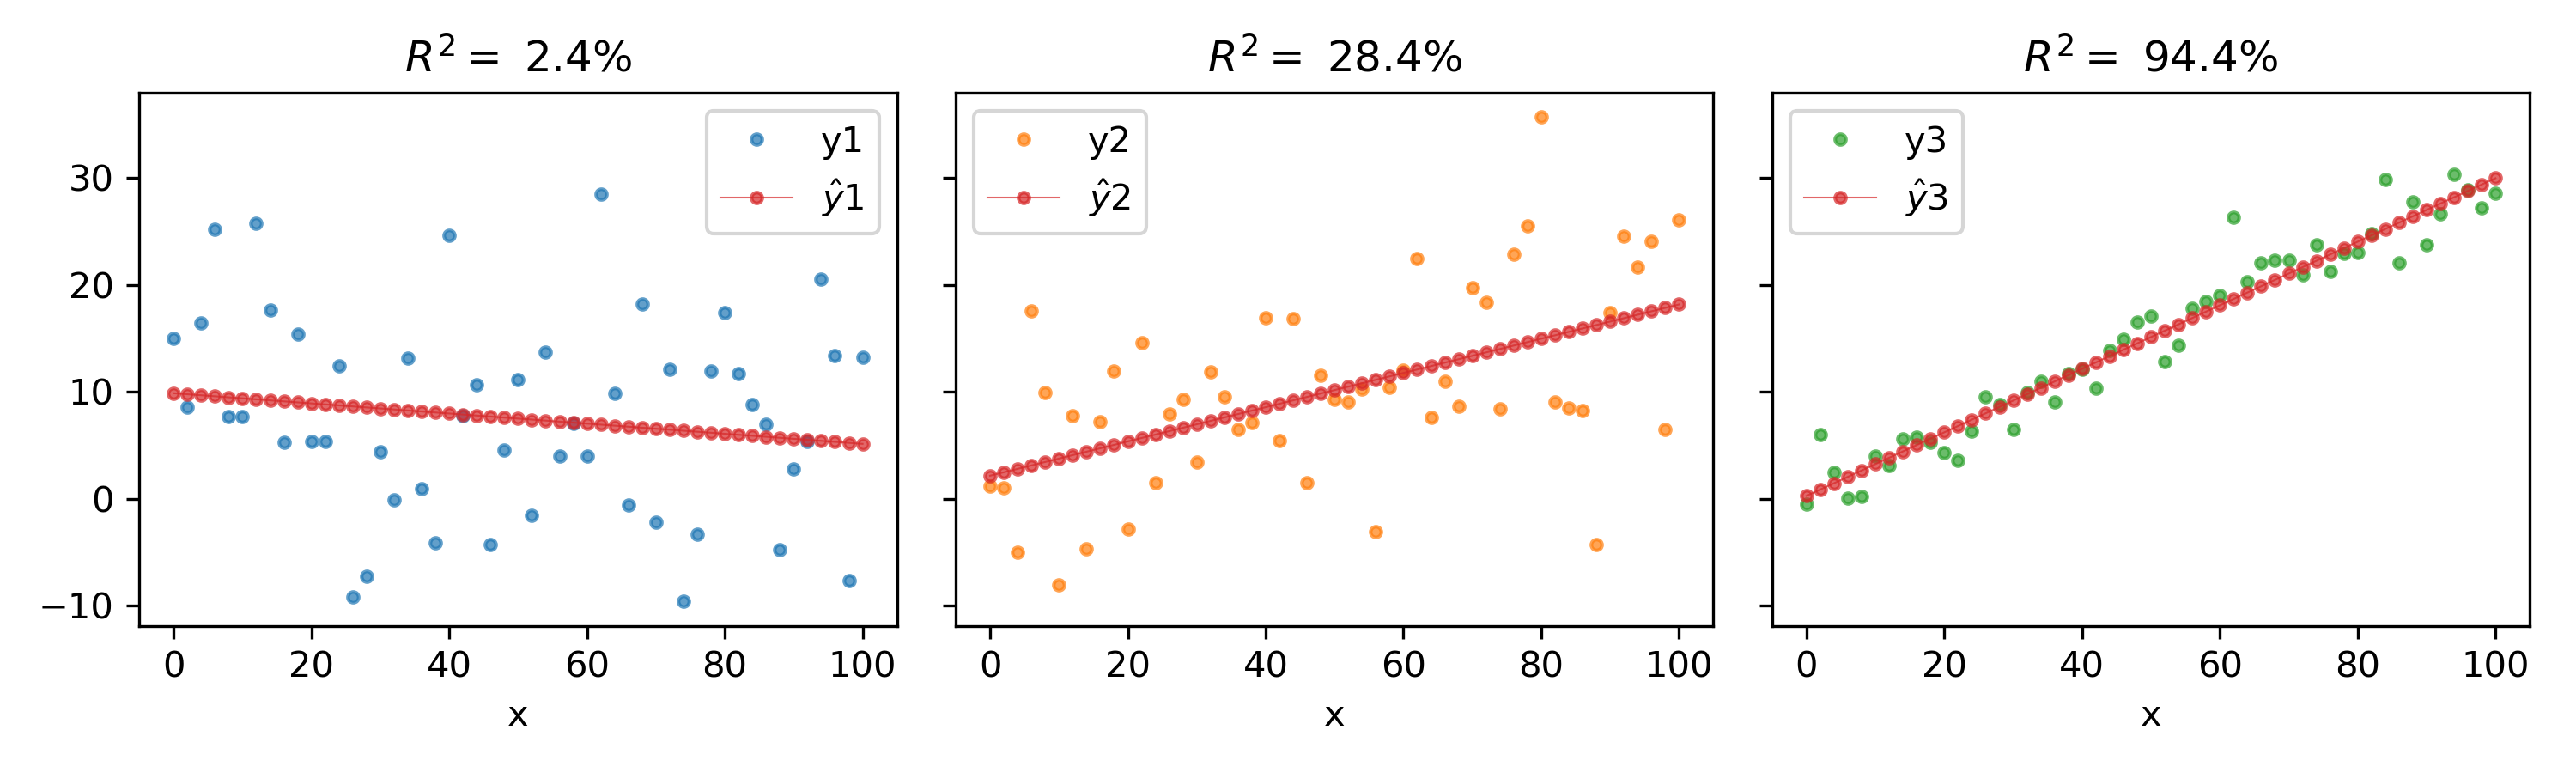
\includegraphics[width=0.98\textwidth]{figures/comparison-rsquared.png}
	\caption{$R^2$: how much is explained by the regression}
	\label{fig:rsquared}
\end{figure}

The higher R-Squared is, the more the data is \textit{explained} or \textit{reflected} in the prediction.
If R-Squared is too small, such as the leftmost case, then it probably indicates that linear regression is not a suitable tool for this problem.
The rightmost case is usually \textit{too good to be true} for most of the complex problems in real-world.
Most of the time, especially for data involve human behavior like economics, R-Squared of around 30\% is often considered to be good. 

Back to our task, now we can define out task as to find $w$ that achieves the highest R-Squared possible.
Since $SS_T$ is a constant value of a problem which only involves $y$ and $\bar y$ regardless the choice of our model, our task is then simply to minimize $SS_E$.

\section{How do we minimize $SS_E$?}
As we explained above, $SS_E$ indicates the distance between our model and perfection, and thus we would like to minimize it.
\begin{equation}
SS_E = \sum_{i = 1}^n (y_i - \hat y_i) ^2
\end{equation}
where $\hat y_i$ is the predicted outcome from our model
\begin{equation}
\hat y_i = w_0 + x_{i, 1}w_1 + x_{i, 2}w_2 + ... + x_{i, k}w_k = \sum_{j=0} ^k x_{i, j}w_j
\end{equation}

Therefore, $SS_E$ is written as
\begin{equation}
SS_E = \sum_{i = 1}^n (y_i - \sum_{j=0} ^k x_{i, j}w_j) ^2
\end{equation}

The problem is then: given $x_{i, j}$ and $y_i$, find $w_j$ that minimize $SS_E$.
This is one example of optimization problems, which can be solved by many methods.
For linear regression, there is one particular effective method: \textit{gradient descent}.

The basic idea of gradient descent it to find the derivative or gradient between $SS_E$ and $w_j$, and gradually changing $w_j$ to the desired direction.
In other words, if increase of $w_j$ would decrease $SS_E$, we will increase $w_j$ by a little bit. 
In contrast, if increase of $w_j$ would increase $SS_E$, we will instead  decrease $w_j$ by a little bit. 
\begin{equation}
\begin{split}
\frac{\partial SS_E}{\partial w_j} & = \frac{\partial}{\partial w_j} \sum_{i = 1}^n (y_i - \hat y_i) ^2 \\
&= \frac{\partial}{\partial w_j}\sum_{i = 1}^n (y_i - \sum_{j=0} ^k x_{i, j}w_j) ^2\\
& = \sum_{i = 1}^n \left[-2(y_i - \sum_{j=0} ^k x_{i, j}w_j)  \frac{\partial}{\partial w_j}\sum_{j=0} ^k x_{i, j}w_j \right]\\
& = \sum_{i = 1}^n \left[ -2(y_i - \sum_{j=0} ^k x_{i, j}w_j)  x_{i, j}\right] \\
& = -2\sum_{i = 1}^n\left[(y_i - \hat y_i)  x_{i, j}\right]\\
\end{split}
\end{equation}

This can also be written as 
\begin{equation}
\begin{split}
\frac{\partial SS_E}{\partial w_j} & =-2\sum_{i = 1}^n\left[(y_i - \hat y_i)  x_{i,j}\right]\\
&=-2\left[(y_1 - \hat y_1)  x_{1,j} + (y_2 - \hat y_2)  x_{2,j} + ... + (y_n - \hat y_n)  x_{n,j}\right]\\
\end{split}
\end{equation}

In matrix expression, this is
\begin{equation}
\frac{\partial SS_E}{\partial w_j} = -2 (Y - \hat Y)X
\end{equation}

We can verify this expression as 
\begin{equation}
\begin{split}
\begin{bmatrix}\frac{\partial SS_E}{\partial w_0} \\ \\ \frac{\partial SS_E}{\partial w_1} \\ \\  \frac{\partial SS_E}{\partial w_2}  \\ \\ ... \\  \\ \frac{\partial SS_E}{\partial w_k}\end{bmatrix}
& = -2 \begin{bmatrix}y_1 - \hat y_1 & y_2 - \hat y_2 & ... & y_n - \hat y_n\end{bmatrix}
\begin{bmatrix}
1 & x_{1, 1} & x_{1, 2} & ... & x_{1, k} \\
1 & x_{2, 1} & x_{2, 2} & ... & x_{2, k} \\
... & ... & ... & ... & ... \\
1 & x_{n, 1} & x_{n, 2} & ... & x_{n, k} \\
\end{bmatrix}\\
& = -2 \begin{bmatrix}
(y_1 - \hat y_1)\times 1  + (y_2 - \hat y_2) \times 1 + ... + (y_n - \hat y_n) \times 1 \\
(y_1 - \hat y_1)  x_{1,1} + (y_2 - \hat y_2)  x_{2,1} + ... + (y_n - \hat y_n)  x_{n,1}\\
(y_1 - \hat y_1)  x_{1,2} + (y_2 - \hat y_2)  x_{2,2} + ... + (y_n - \hat y_n)  x_{n,2}\\
...\\
(y_1 - \hat y_1)  x_{1,k} + (y_2 - \hat y_2)  x_{2,k} + ... + (y_n - \hat y_n)  x_{n,k}\\
\end{bmatrix}
\end{split}
\end{equation}

One we get $\frac{\partial SS_E}{\partial w_j}$, we then update $w_j$ accordingly.
If $\frac{\partial SS_E}{\partial w_j} > 0$, this indicates an increase of $w_j$ would increase $SS_E$.
Therefore we should decrease $w_j$ as the following:
\begin{equation}
w_j = w_j - \alpha \frac{\partial SS_E}{\partial w_j} 
\end{equation}
where $\alpha$ is an arbitrary coefficient to represent how far we want $w_j$ to move along the desired direction.
 
In contrast, if $\frac{\partial SS_E}{\partial w_j} < 0$, this indicates an increase of $w_j$ would decrease $SS_E$.
Therefore we should increase $w_j$ as the following:
\begin{equation}
w_j = w_j - \alpha \frac{\partial SS_E}{\partial w_j} 
\end{equation}
Notice in this equation, since $\frac{\partial SS_E}{\partial w_j} < 0$, $w_j$ minus $\frac{\partial SS_E}{\partial w_j}$ is in fact increasing $w_j$.

This is one step of gradient descent. 
To find the optimal $w$, we iterate over and over again, moving $w_j$ along the desired direction bit by bit from iteration to iteration.
Eventually, every $w_j$ converges to its optimal value.
To decide if gradient descent is converged, we can monitor the value of $SS_E$.
If $SS_E$ does not decrease from iteration to iteration or if the decrease is too small, we can conclude the iterations are converged and there is no need to continue updating $w$.

\section{Implement gradient descend in Python}
To implement linear regression and gradient descent in Python, first we construct a class called \textit{LinearRegression}.
The variable \textit{max\_iteration} represents the allowable number of iterations so that the iterations would not run forever.
The variable \textit{tol} represents the tolerance of meaningful decrease of $SS_E$ from one iteration to the next.
If the decrease is less than this tolerance, then we conclude the decrease is not considerable anymore and we stop the iteration.
\begin{lstlisting}
class LinearRegression:
    def __init__(self, x, y, max_iteration=1000, tol=1e-3):
        self.max_iteration = max_iteration
        self.tol = tol
        
    def gradient_descend(self, x, y, lr=0.01):
        # Get number of instances (n) and number of attributes (d)
        n = x.shape[0]
        d = x.shape[1]

        # Initialize weights and bias with zeros
        w = np.zeros(d)

        # Initialize list to store MSE
        mse_log = []

        # Loop for gradient descent
        for i in range(self.max_iteration):
            y_pred = np.matmul(x, w)
            mse = np.mean((y - y_pred) ** 2)

            # Terminate if decrease of MSE is less than tol
            if len(mse_log) != 0 and 0<=(mse_log[-1]-mse)/mse_log[-1]<self.tol:
                break
            elif len(mse_log) != 0 and mse_log[-1] < mse:
                break
            else:
                mse_log.append(mse)

            gradient_w = -2 * np.matmul((y - y_pred), x) / n
            w -= lr * gradient_w

        return w, mse_log
\end{lstlisting}

One difference between the previous equations and the code is that we use $MS_E$ in the code rather than $SS_E$.
In the code, $MS_E$ is simply calculated as $\frac{SS_E}{n}$.
As $n$ is a constant for given data, the derivative of $MS_E$ to $w$ is then
\begin{equation}
\frac{\partial MS_E}{\partial w_j} = -\frac{2}{n} (Y - \hat Y)X
\end{equation}
In the code, this is implemented as 
\begin{lstlisting}
 gradient_w = -2 * np.matmul((y - y_pred), x) / n
\end{lstlisting}

Another note is that the coefficient $\alpha$ is often called \textit{learning rate} in machine learning, which is the variable \textit{lr} in the code. 
Choosing proper learning rate is crucial for a successful linear regression.
We will talk about how we can actually determine learning rate later in this post.

\section{Visualization of gradient descent}
Let's use the third example data set to visualize gradient descent.
For now, suppose we can somehow magically determine the proper learning rate.

In this example, the learning rate $\alpha$ is set as 0.007 for $w_0$ and 0.0001 for $w_1$.
At the beginning, we do not know much about $w$, so one method to initialize is to set all $w_j$ to be zero.
In our example, this means we start with $\hat y = 0 x + 0$.
In this case, we are far away from the true $y$ with a $SS_E$ of 15960.
We calculated the gradient of $w_j$ using
\begin{equation}
\frac{\partial MS_E}{\partial w_j} = -\frac{2}{n} (Y - \hat Y)X
\end{equation}
In this example,
\begin{equation}
\begin{split}
\frac{\partial MS_E}{\partial w_0} &= -30.406\\
\frac{\partial MS_E}{\partial w_1} &= -2037.650\\
\end{split}
\end{equation}
\begin{figure}[htbp]
	\centering
	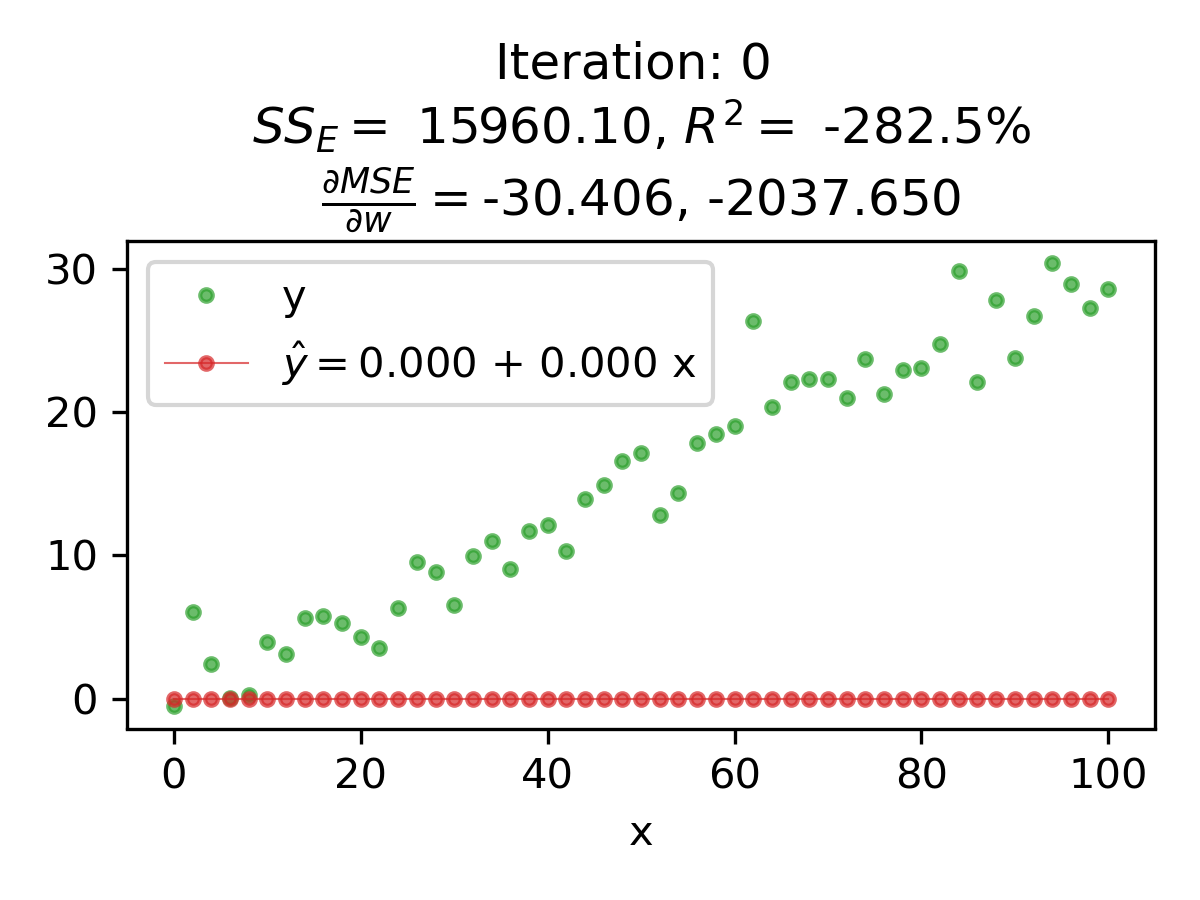
\includegraphics[width=0.6\textwidth]{figures/visualize-0.png}
	\caption{Iteration 0 of gradient descent}
	\label{fig:vis0}
\end{figure}

We need to update $w_j$ to the direction that decrease $MS_E$.
\begin{equation}
\begin{split}
w_0 &= w_0 - \alpha_0 \frac{\partial MS_E}{\partial w_0} = 0 - 0.007\times (-30.406) = 0.213\\
w_1 &= w_1 - \alpha_ 1 \frac{\partial MS_E}{\partial w_1} = 0 - 0.0001\times (-2037.650)=0.204 \\
\end{split}
\end{equation}

Now our model becomes $\hat y = 0.213 + 0.204 x$.
We move forward to the next iteration. 
With this new $\hat y$, our $SS_E$ is reduced to 1807, indicating we are moving along the correct direction.
\begin{figure}[htbp]
	\centering
	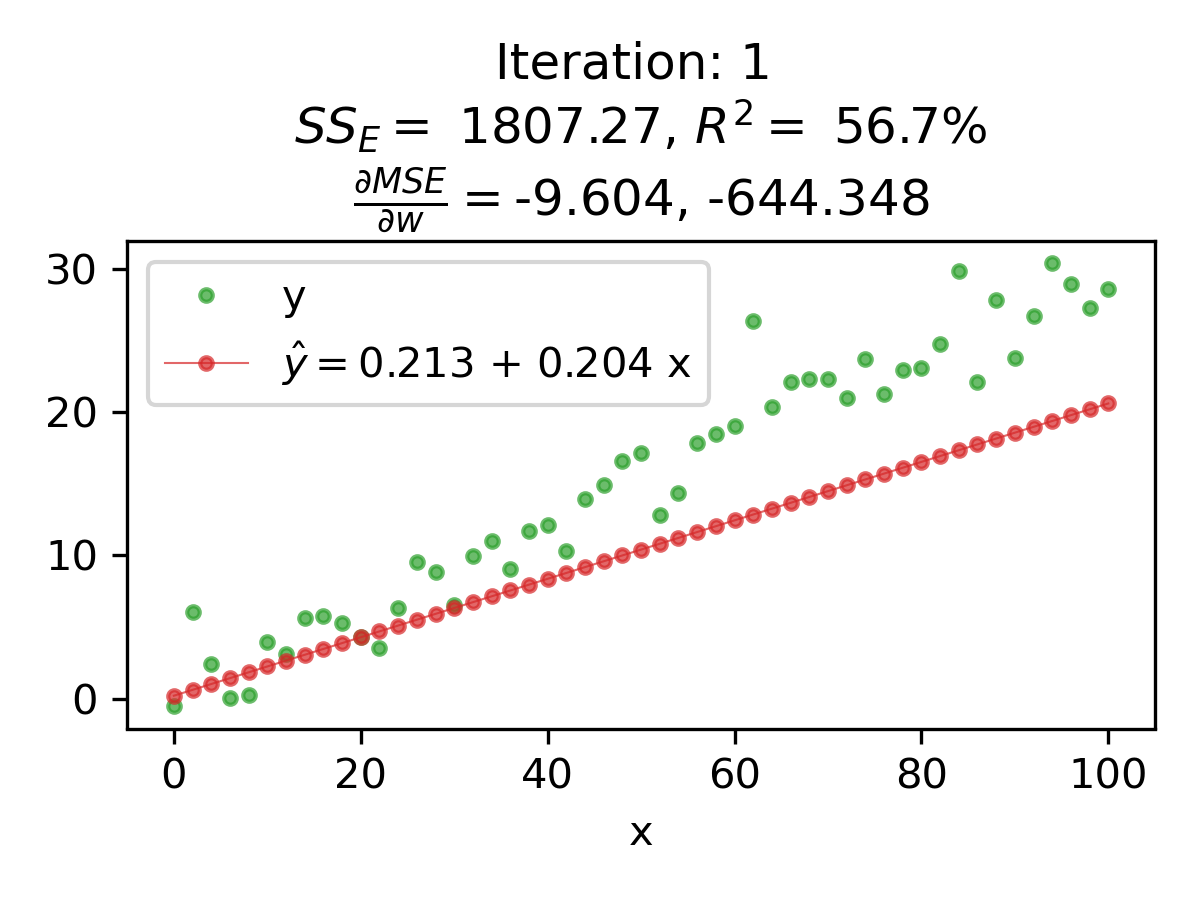
\includegraphics[width=0.6\textwidth]{figures/visualize-1.png}
	\caption{Iteration 1 of gradient descent}
	\label{fig:vis1}
\end{figure}

Again, we update $w_j$in this iteration.
\begin{equation}
\begin{split}
w_0 &= w_0 - \alpha_0 \frac{\partial MS_E}{\partial w_0} = 0.213 - 0.007\times (-9.604) = 0.280\\
w_1 &= w_1 - \alpha_ 1 \frac{\partial MS_E}{\partial w_1} = 0.204 - 0.0001\times (-644.348)=0.268 \\
\end{split}
\end{equation}

After this iteration, our model becomes $\hat y = 0.280 + 0.268 x$, our $SS_E$ is reduced to 392, and we achieve a R-Squared over 90\%.
It feels pretty good.
Let us move on to next iteration.
\begin{figure}[htbp]
	\centering
	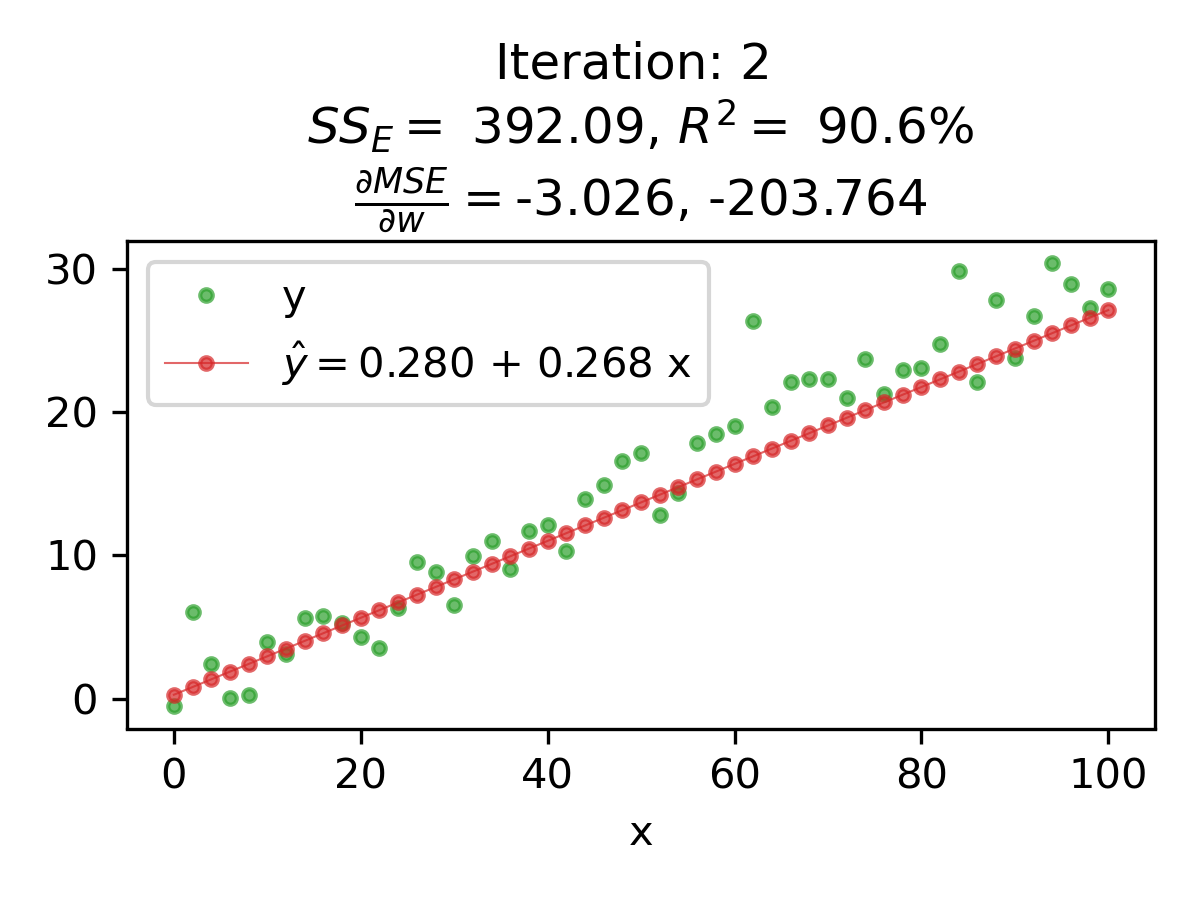
\includegraphics[width=0.6\textwidth]{figures/visualize-2.png}
	\caption{Iteration 2 of gradient descent}
	\label{fig:vis2}
\end{figure}

Again, we update $w_j$ in this iteration.
\begin{equation}
\begin{split}
w_0 &= w_0 - \alpha_0 \frac{\partial MS_E}{\partial w_0} = 0.280 - 0.007\times (-3.026) = 0.301\\
w_1 &= w_1 - \alpha_ 1 \frac{\partial MS_E}{\partial w_1} = 0.268 - 0.0001\times (-203.764)=0.289 \\
\end{split}
\end{equation}

Now our model becomes $\hat y = 0.301 + 0.289 x$, our $SS_E$ is reduced to 250, and we achieve a R-Squared of 94\%.
The fitted line of $\hat y$ looks reasonable along the actual $y$.
If we feel comfortable with this result, we can just stop here.
\begin{figure}[htbp]
	\centering
	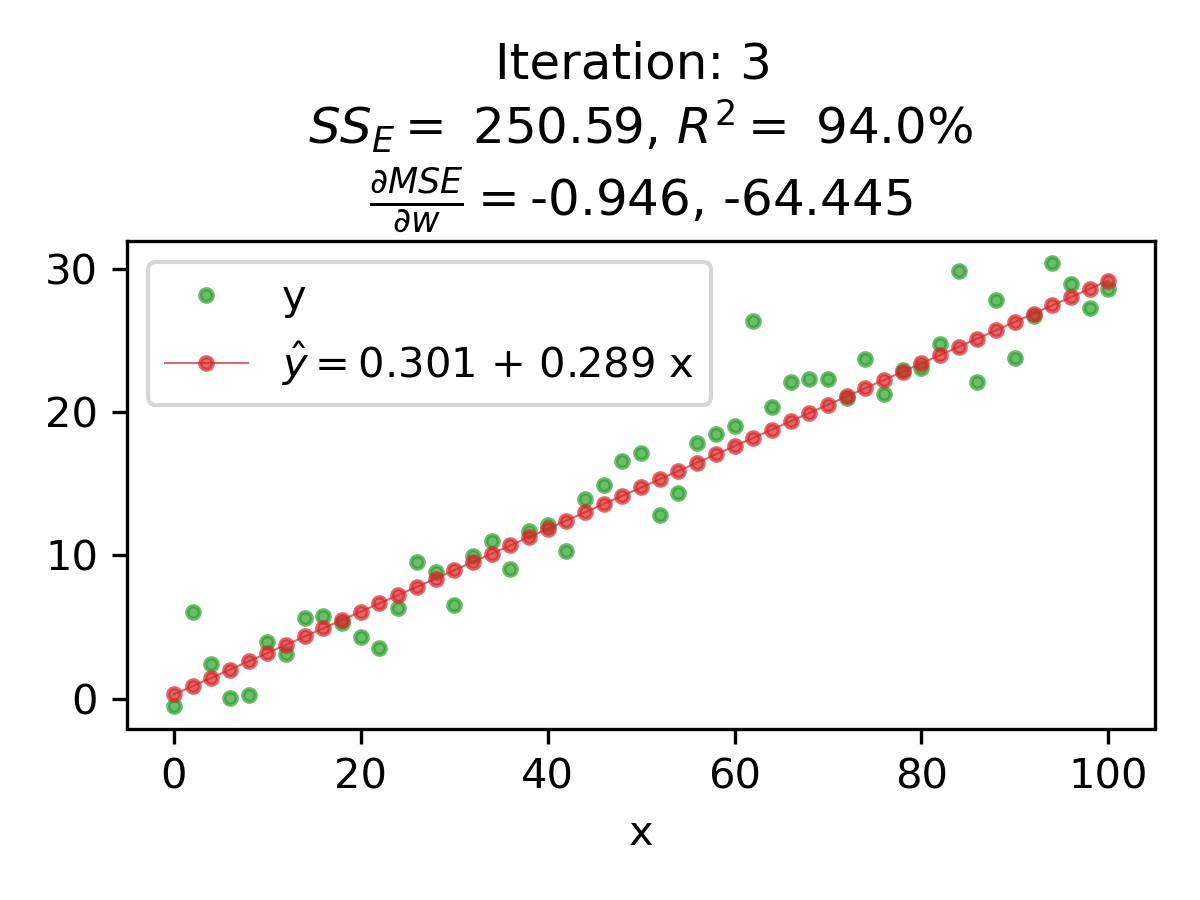
\includegraphics[width=0.6\textwidth]{figures/visualize-3.png}
	\caption{Iteration 3 of gradient descent}
	\label{fig:vis3}
\end{figure}

In this deliberately designed example, we achieved a pretty good linear regression model within just 3 iterations.
Of course this is too good to be true for most real-world problems.
To solve real-world problems, we have to examine how to choose a proper learning rate.

\section{What is a proper learning rate?}
In the previous section, we somehow magically get the learning rate for $w_j$.
But we haven't talk about how to choose learning rate yet, so our next question is what is a proper learning rate?
In gradient descent, we use learning rate $\alpha$ to update weights $w$.
To successfully and effectively converge to an optimal solution, learning rate has to be proper.
Figure~\ref{fig:difflr} illustrates the effects of different learning rates on one particular example data set.
Different learning rates start from the same initial MSE but result in different learning behaviors.
\begin{figure}[htbp]
	\centering
	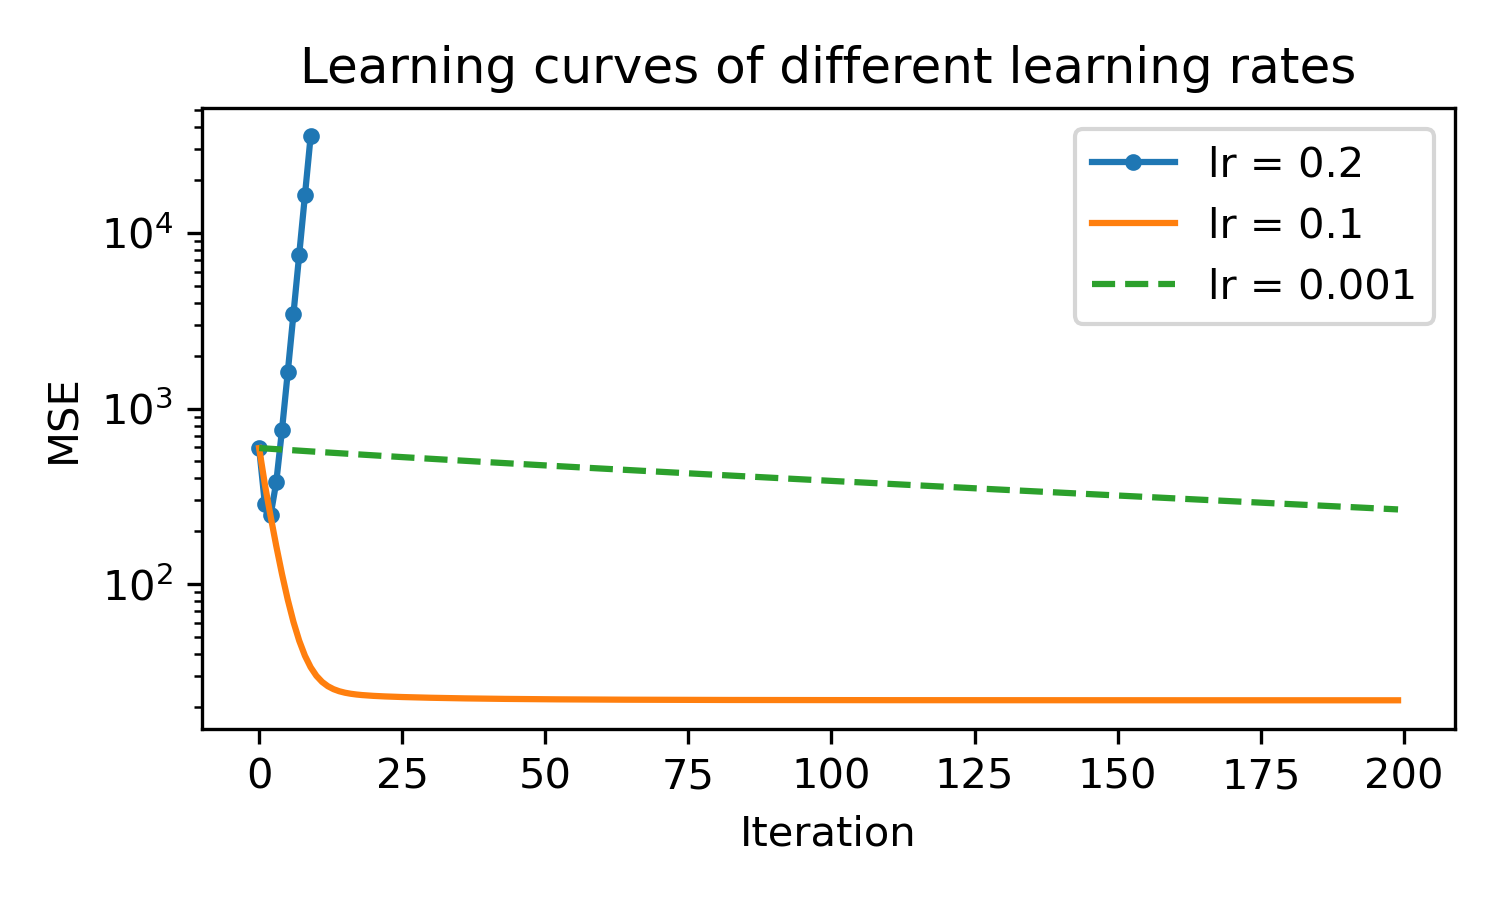
\includegraphics[width=3.5 in]{figures/diff-learning-rates.png}
	\caption{Learning curves of different learning rates}
	\label{fig:difflr}
\end{figure}

If learning rate is too small, such as the curve corresponding to learning rate of 0.001, the learning process is unnecessarily slow and the iterations do not converge within the given allowable number of iterations.
On the other hand, if learning rate is too large, then the learning process may become unstable as shown by the curve corresponding to learning rate of 0.2.
The basic assumption of partial derivative in calculus is that it is only applicable to a small region near that point, not applicable to regions far away from the point.
Therefore, learning rate should be kept small enough so that the movement is within that region.
In summary, learning rate needs to be a sweet spot, not too small nor too large, like the curve corresponding to learning rate of 0.1.

In our code, we use an automatic process to tune learning rate. 
We first start with a learning rate of 0.1, then we try 0.01, 0.001, and so on.
We stop when the MSE achieved by a learning rate is more than 10 times larger than that of the previous learning rate.
Then the learning rate corresponding to the minimum MSE is chosen as the optima learning rate.
\begin{lstlisting}
    def tune_learning_rate(self):
        lr = 0.1
        w, mse_log = self.gradient_descend(self.x_train, self.y_train, lr=lr)
        lr_list = [lr]
        mse_list = [mse_log[-1]]

        while lr > 1e-20:
            lr *= 0.1
            w, mse_log = self.gradient_descend(self.x_train, self.y_train, lr=lr)
            # if mse is 10 times larger than previous iteration, stop
            if mse_log[-1] > 10 * mse_list[-1]:
                break
            lr_list.append(lr)
            mse_list.append(mse_log[-1])

        opt_lr = lr_list[mse_list.index(min(mse_list))]

        return opt_lr
\end{lstlisting}

\section{Scale data before training}
For linear regression, it is not required to use scaled data.
However, our code still scales and centers data before training.

The first reason is that this helps our autonomous tuning of learning rate.
If the data are not scaled, the numerical range of different attributes may be significantly different and thus the proper learning rate for each attribute may be considerably different.
By scaling $x$, we are able to apply the same learning rate on all data attribute. 

The second reason is that several advanced methods, which are based on linear regression, such as LASSO, rigid regression, and elastic net, require the data to be scaled.
To use our code as the foundation of these methods in the further, we apply data scaling and centering in our code.
\begin{lstlisting}
class LinearRegression:
    def __init__(self, x, y, max_iteration=1000, tol=1e-3):
        self.max_iteration = max_iteration
        self.tol = tol
        
        self.x_raw = x
        self.mu = np.mean(x, axis=0)
        self.sigma = np.std(x, axis=0)
        self.x_train = self.standard_transform(x)
        self.y_train = y
        self.weights = None
        
    def standard_transform(self, x):
        scaled_x = (x - self.mu) / self.sigma
        scaled_x = np.insert(scaled_x, 0, np.ones(scaled_x.shape[0]), axis=1)
        return scaled_x
\end{lstlisting}

In this function, besides scaling and centering, we also insert a column of 1 as the first column of $X$ so that we have a single $w$ vector without using an additional variable of $b$ for bias.

\section{API of the learner}
We use the following API to train and utilize the learner.
\begin{lstlisting}
    def fit(self, lr=None):
        if lr is None:
            lr = self.tune_learning_rate()
        w, mse_log = self.gradient_descend(self.x_train, self.y_train, lr=lr)
        self.weights = w
    
    def predict(self, x):
        x_test = self.standard_transform(x)
        return np.matmul(x_test, self.weights)
\end{lstlisting}
If user specifies a learning rate, that learning rate is used in gradient descent. Otherwise, the code determines a proper learning rate by calling the \textit{tune\_learning\_rate function}.

Because we scaled training data before gradient descant, the weights are corresponds to the scaled data. 
As a result, when we utilize the learner on new test data, these new test data need to be scaled the same way.

Using this API, for given training and testing data sets, a learner can be built and trained using the following code. We can then utilize the learner on new testing data and get predicted y of testing x.
\begin{lstlisting}
learner = LinearRegression(x_train, y_train, plot=plot, verbose=True)
learner.fit()
\end{lstlisting}

To utilize the learning on testing data set, we can get predicted y of testing x.
\begin{lstlisting}
y_pred = learner.predict(x)
\end{lstlisting}

\section{Example using \textit{diamonds} data set}
We use \textit{diamonds} data set from \textit{R} package \textit{yarrr} (\url{https://rdrr.io/cran/yarrr/man/diamonds.html}) as an example to run our learner.
This data set has 150 data instances and 3 attributes: weight, clarity scale, and color scale.
The outcome is the value of the diamond.
The first 10 instances of the data set are previewed in the following table:
\begin{table}[htbp]
	\small 
	\centering 
		\caption{Preview of \textit{diamonds} data set}
		\label{table:diamonds}
	\begin{tabular}{r r r|r}
		Weight & Clarity & Color & Value \\
9.35	&		0.88	&		4		&	  182.5\\
11.10	&   1.05	&		5		&  191.2\\
8.65	&		0.85	&		6		&  175.7\\
10.43	&		1.15	& 	5		&  195.2\\
10.62	&		0.92	&		5		&  181.6\\
12.35	&		0.44	&		4		&  182.9\\
11.24	&		1.09	& 	6		&  195.9\\
9.77	&		1.43	&		4		&  188.6\\
11.83	& 	0.95	&		6		&  190.3\\
9.55	&		1.05	&		5		&  190.7\\
...	&		...	&		...		&  ...\\
	\end{tabular}
 \end{table}
 
Using our code, we train a linear regression model for this data set.
\begin{lstlisting}
df = pd.read_csv('data/diamonds.csv', sep=' ')
df = df.to_numpy()
x = df[:, 0:-1]
y = df[:, -1]
learner = LinearRegression(x, y, plot=plot)
learner.fit()
y_pred = learner.predict(x)
\end{lstlisting}

The autonomous tuning of learning rates is shown in Figure~\ref{fig:tune-lr}.
For this data set, learning rate of 0.1 seems to be the optimal choice as it achieved the minimum MSE and uses the smallest number of iterations.
\begin{figure}[htbp]
	\centering
	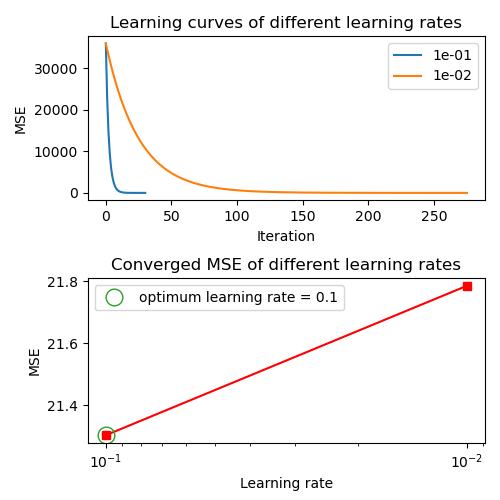
\includegraphics[width=0.5\textwidth]{figures/tune-lr.png}
	\caption{Tune of learning rate for \textit{diamonds} data set}
	\label{fig:tune-lr}
\end{figure}

The results of the model can be visualized by plotting predicted values versus true values in Figure~\ref{fig:res_diamonds}.
The closer our predictions to the true values, the closer these plotted points to the red diagonal line.
As we can see in the figure, the points in training and testing plots generally lay along the diagonal line. 
\begin{figure}[htbp]
	\centering
	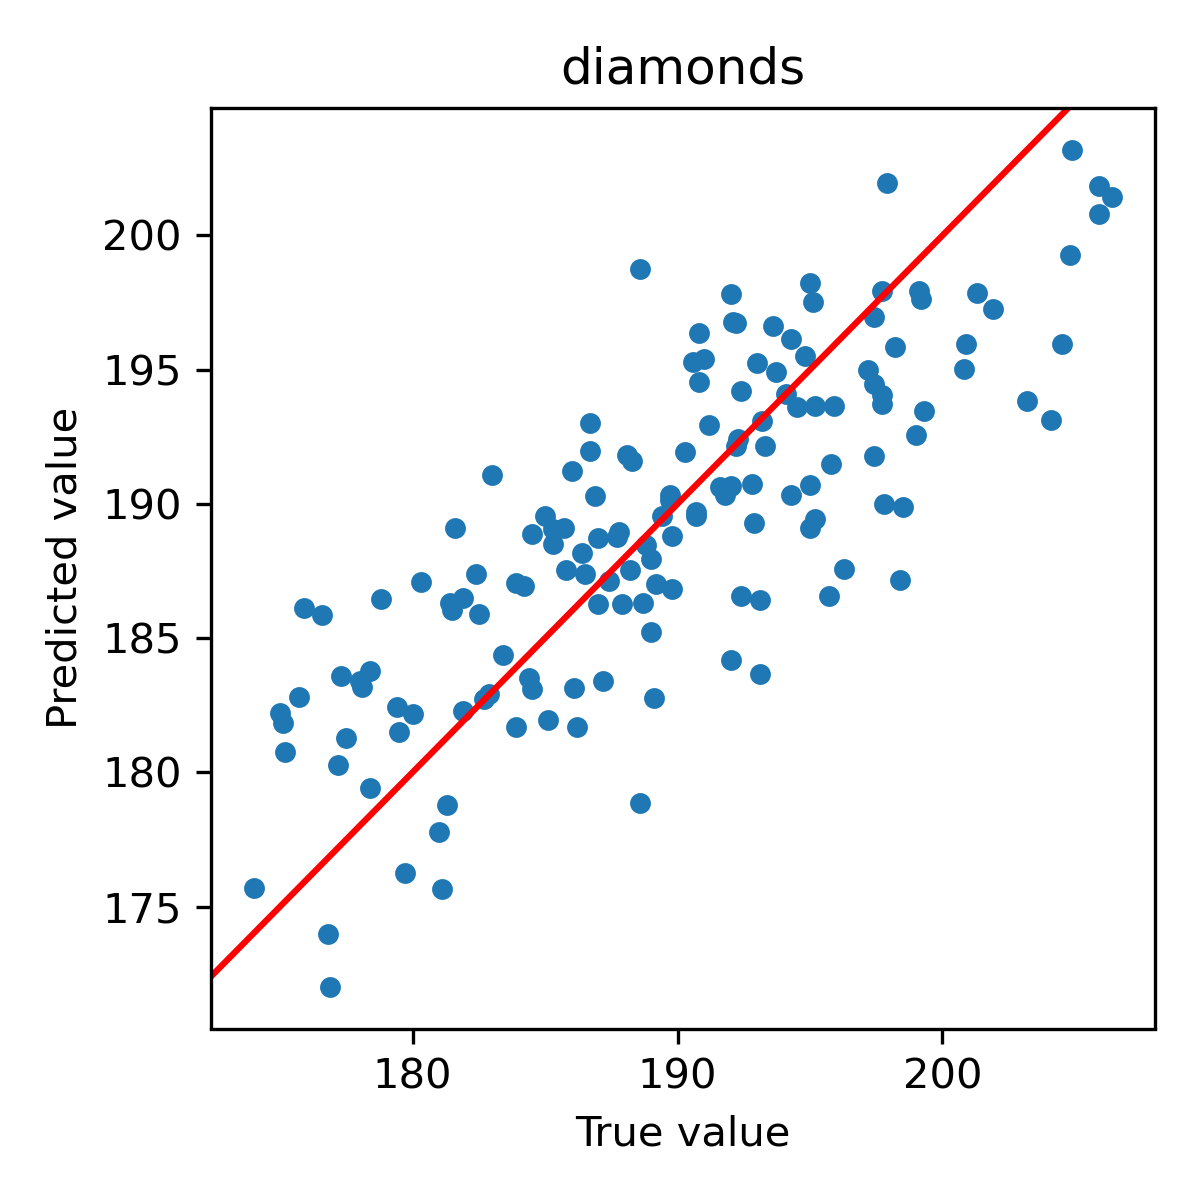
\includegraphics[width=0.5\textwidth]{figures/our-result-diamonds.png}
	\caption{Visualization of predicted values versus true values for \textit{diamonds} data set}
	\label{fig:res_diamonds}
\end{figure}

\section{How do we interpolate the learning?}
Now we have finished our linear regression on this \textit{diamonds} data set. 
Imagine we need to give an elevator pitch to business partners or policy makers, what should we present?
One of the most important outputs of linear regression is the weights of data attributes, which give us insights into the relations between attributes and outcome.

As we did gradient descent on scaled data, out weights also corresponds to the scaled data.
To relate the weights back to original data, we need to do some calculation to derive the weights for unscaled data.
\begin{lstlisting}
def get_unscaled_weights(self):
    unscaled_wights = self.weights[1:] / self.sigma
    unscaled_intercept = self.weights[0]-np.sum(self.weights[1:]*self.mu/self.sigma)
    unscaled_wights = np.insert(unscaled_wights, 0, unscaled_intercept)
    return unscaled_wights
\end{lstlisting}

Using this function, we obtain the weights for each attributes in the \textit{diamonds} data set.
As we explained before, the data outcome, which is the value of diamonds, can be approximated using a linear combination of weights and data attributes:
\begin{equation}
\text{diamond value} = 150.12+ 2.17 (\text{weight}) + 20.67(\text{clarity})-0.63(\text{color})
\end{equation}

For this simple data set, we learn from the weights that the more the weights, the more the value, which seems reasonable.
We also learn that the higher the clarity grade, the more the value, which also makes sense as people prefer diamonds with no or little inclusion or blemish.
For color, the lower the color scale, the more the value, which probably indicates people prefer colorless diamonds.

\section{How confident are we?}
In our elevator pitch, we present the linear equation above and we talk about the relation between value and weight, clarity, or color.
However, there is an important question: how sure are we?
In statistics words, is our model significant enough?

To answer this question, we can perform a \textit{significance test}.
We still use $n$ as the number of data instances and $k$ as the number of data attributes.
We already talked about $SS_T$, $SS_R$, and $SS_E$.
One indicator is R-Squared which is already covered previously
\begin{equation}
R^2 = 1 - \frac{SS_E}{SS_T} = \frac{SS_R}{SS_T}
\end{equation}

One drawback of using R-Squared is that it is compromised by increasing number of attributes.
If the number of attributes is huge, then we can find $w$ that generate a very small $SS_E$ and thus a very high R-Squared.
However, this does not always indicate that our model is perfect.
As there are so many random effects in these huge numbers of attributes, the model captures almost all of these random effects to achieve a high R-Squared.
In machine learning, this is an example of \textit{overfitting}.
To overcome this, we introduce an adjusted version of R-Squared to deal with this.

To determine adjusted R-Square, we first define the corresponding mean of sum of squares.
\begin{equation}
MS_T = \frac{SS_T}{n-1}
\end{equation}
\begin{equation}
MS_R = \frac{SS_T}{k}
\end{equation}
\begin{equation}
MS_E = \frac{SS_E}{n-(k+1)}
\end{equation}

Then the adjusted R-Squared is defined as
\begin{equation}
R_{\text{adjusted}}^2 = 1 - \frac{MS_E}{MS_T}
\end{equation}

The relation between R-Squared and adjusted R-Squared can be derived.
\begin{equation}
\begin{split}
R_{\text{adjusted}}^2 &= 1 - \frac{MS_E}{MS_T}\\
& =  1 - \frac{\frac{SS_E}{n-(k+1)}}{\frac{SS_T}{n-1}}\\
& = 1 - \frac{n-1}{n-(k+1)} \frac{SS_E}{SS_T}\\
& = 1 - \frac{n-1}{n-(k+1)} (1-R^2)
\end{split}
\end{equation}

We can see that adjusted R-Squared decreases as $k$ increases.
In some sense, we can say adjusted R-Squared encourages models with smaller number of data attributes.
In other words, if two models achieve same R-Squared, but one with a significantly smaller number of attributes, then this one will have a smaller adjusted R-Squared and thus is preferable than the other one.

R-Squared and adjusted R-Squared can be calculated using the following code.
\begin{lstlisting}
y = self.y_train
y_pred = np.matmul(self.x_train, self.weights)

n = self.x_train.shape[0]
k = self.x_train.shape[1] - 1

ss_total = np.sum((y - np.mean(y)) ** 2)
ms_total = ss_total / (n - 1)

ss_regression = np.sum((y_pred - np.mean(y)) ** 2)
ms_regression = ss_regression / k

ss_error = np.sum((y - y_pred) ** 2)
ms_error = ss_error / (n - k - 1)

r_square = 1 - ss_error / ss_total
adj_r_square = 1 - ms_error / ms_total
\end{lstlisting}

In our \textit{diamonds} example, the R-Squared turns out to be 63.67\% and the adjusted R-Squared turns out to be 62.92\%.

Now we are ready to perform the significance test.
For linear regression, we usually use a F-test to assess the significance.
The \textit{F-statistic} is defined as the ratio between the \textit{explained} variances to \textit{unexplained} variances.
\begin{equation}
F = \frac{MS_R}{MS_E}
\end{equation}

Using this \textit{F-statistic}, we can then determine the corresponding $P$ value.
To do that, first we need to determine the degree of freedom (dof) of the F-distribution.
In linear regression, the first dof is $k$ and the second dof is $n - (k+1)$.
In our \textit{diamonds} example, we are looking at first dof of 3 and second dof of 146.
The F-distribution and the corresponding survival function is plotted in the Figure~\ref{fig:f-test}.
\begin{figure}[htbp]
	\centering
	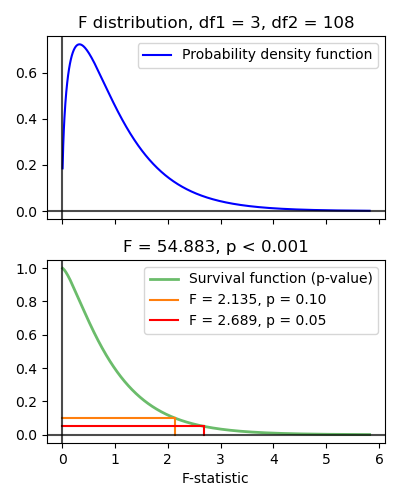
\includegraphics[width=0.5\textwidth]{figures/f-test.png}
	\caption{F-test of linear regression on \textit{diamonds} data set}
	\label{fig:f-test}
\end{figure}

When $F=2.689$, the area under the probability density curve on the right side of 2.689 is 0.05, indicating a $F$ value of 2.689 corresponds to a $P$ value of 0.05.
Similarly, the area under the probability density curve on the right side of 2.135 is 0.10, indicating a corresponding $P$ value of 0.10.
In our \textit{diamonds} example, our $F$ turns out to be 85.293, which is way on the right side of our plot.
As a result, the corresponding P-value is extremely small.

P-value has strict definitions in statistics which we will not go into details today.
What we need to know is that P-value indicates the probability that the reason why our model performs this well is purely by luck.
In this case, this probability is very low, definitely smaller than 0.001.
In statistics, 0.05 is usually used as the threshold.
As a result, we conclude that this is not caused by pure luck, and thus, our model is at least somewhat ``meaningful'', which is called ``significant'' in statistics.

\section{Is every attribute relevant?}
One final question we need to address is whether every attribute is relevant.
By relevant, we mean ``meaningfully contribute'' to the outcome.
If a certain attribute is random values not related to the outcome at all, we call that attribute irrelevant.
For example, imagine we add a column of ``weather of New York City when this diamond was produced'' to the \textit{diamonds} data set, this data attribute probably would not affect the value of diamonds at all.
How do we identify if there is any irrelevant attribute?

Let us look back at our math expressions.
This time we express everything as vectors and matrix.
We are looking for a vector of weights $w$ that linearly relates $X$ to $Y$ as close as possible.
The ``closeness'' can be expressed as the sum square of error $SS_E$.
\begin{equation}
SS_E = \sum_{i = 1}^n (y_i - \hat y_i) ^2
\end{equation}
Written as matrix, this equation is 
\begin{equation}
SS_E = (Y - \hat Y)^T (Y - \hat Y)
\end{equation}
The predicted outcome $\hat Y$ of our model is obtained by
\begin{equation}
\hat Y =  X w
\end{equation}
Therefore, 
\begin{equation}
\begin{split}
SS_E & = (Y - X w)^T (Y - X w)\\
 & = (Y^T -  w^TX^T)(Y- X w)\\
 & = Y^TY -Y^TX w - w^TX^TY + w^TX^T X w\\
\end{split}
\end{equation}
For the second term and the third term, we can find that they are transpose of each other.
\begin{equation}
(Y^T X w)^T = w^T X^T Y
\end{equation}
We then look at the dimensions of these items:
$Y^T$ is $1\times n$, $X$ is $n\times k$, and $w$ is $k \times 1$.
Therefore $Y^T X w$ is $1\times 1$.
For a $1\times 1$ matrix, its transpose is itself.
\begin{equation}
Y^T X w = w^T X^T Y
\end{equation}
Therefore,
\begin{equation}
\begin{split}
SS_E & = Y^T Y -Y^T X w - w^T X^T Y + w^T X^T X w\\
& = Y^T Y - 2w^T X^T Y + w^T X^T X w\\
\end{split}
\end{equation}

Following the principle of gradient descent, we look at the gradient between $SS_E$ and $w$.
\begin{equation}
\begin{split}
\nabla SS_E(w) & = \nabla Y^T Y - 2 \nabla w^T X^T Y + \nabla w^T X^T X w\\
& = 0 - 2X^T Y + 2 \\
& = 2(X^T X w - X^T Y )\\
\end{split}
\end{equation}

To achieve the minimum $SS_E$, we need the gradient to be zero.
\begin{equation}
X^T X w - X^T Y = 0
\end{equation}

We then solve this equation for $w$.
The $w$ that makes the gradient to be zero is usually called $\hat w$.
In other words, among all possible $w$, $\hat w$ is the one that makes $\hat Y = Xw$ as close to $Y$ as possible.
\begin{equation}
X^T X \hat w = X^T Y
\end{equation}
\begin{equation}
 (X^T X)^{-1} X^T X \hat w= (X^T X)^{-1} X^T Y
\end{equation}
\begin{equation}
\hat w= (X^T X)^{-1}X^T Y
\end{equation}


Put $\hat w$ into the equation, we can get
\begin{equation}
\hat Y = X\hat w= X(X^T X)^{-1}X^T Y=HY
\end{equation}
where
\begin{equation}
H= X(X^T X)^{-1}X^T
\end{equation}

Here we have a transformation from $Y$ to $\hat Y$.
\begin{equation}
\hat Y  = HY
\end{equation}
Some people call $H$ the \textit{hat matrix} as it puts the hat on $Y$.

The term $(X^T X)^{-1}$ corresponds to the variances of $w$ and is usually denoted as $C$.
\begin{equation}
C = MS_E (X^T X)^{-1}
\end{equation}

In our \textit{diamonds} example, the covariance matrix turns out to be
\begin{equation}
\begin{split}
C &= MS_E (X^T X)^{-1}\\
& = 21.87
\begin{bmatrix}
0.6020 & -0.0186 & -0.2190 & -0.0387\\
-0.0186 & 0.0018 & -0.0014 & 0.0004\\
-0.2190 & -0.0014 & 0.2103 & 0.0046\\
-0.0387 & 0.0004 & 0.0046 & 0.0061
\end{bmatrix}\\
& = 
\begin{bmatrix}
13.164 & -0.408 & -4.789 & -0.846\\
-0.408 & 0.040 & -0.031 & 0.008\\
-4.789& -0.031 & 4.599 & 0.101\\
-0.846 & 0.008 & 0.101 & 0.133
\end{bmatrix}\\
\end{split}
\end{equation}

The diagonal elements of $C$ represent the standard deviation ($se$) of $w$.
For each weight $w_j$, we have
\begin{equation}
se(w_j)= \sqrt{C_{j,j}}
\end{equation}

Now we can perform a T-test on every $w_j$.
\begin{equation}
t_0 = \frac{w_j}{se(w_j)}
\end{equation}

We already know our weights are 
\begin{equation}
\begin{split}
w &=\begin{bmatrix}
w_0 & w_1 & w_2 & w_3
\end{bmatrix}\\
&=\begin{bmatrix}
148.23 & 2.19& 21.67 & -0.46
\end{bmatrix}\\
\end{split}
\end{equation}

Therefore,
\begin{equation}
\begin{split}
t_0 &=\begin{bmatrix}
\frac{w_0}{se(w_0)} & \frac{w_1}{se(w_1)} & \frac{w_2}{se(w_2)} & \frac{w_3}{se(w_3)}
\end{bmatrix}\\
&=\begin{bmatrix}
\frac{w_0}{\sqrt{C_{0,0}}} & \frac{w_1}{\sqrt{C_{1,1}}} & \frac{w_2}{\sqrt{C_{2,2}}} & \frac{w_3}{\sqrt{C_{3,3}}}
\end{bmatrix}\\
&=\begin{bmatrix}
\frac{148.23}{\sqrt{13.164}} & \frac{2.19}{\sqrt{0.040}} & \frac{21.67}{\sqrt{4.599}} & \frac{-0.46}{\sqrt{0.133}}
\end{bmatrix}\\
&=\begin{bmatrix}
40.85 & 10.93& 10.10 & -1.26
\end{bmatrix}\\
\end{split}
\end{equation}

We then perform a t-test.
As shown in the following figure, for a two-tailed t-test, a critical p-value of 0.05 corresponds to a $t0$ value of 1.976 or -1.976.
\begin{figure}[htbp]
	\centering
	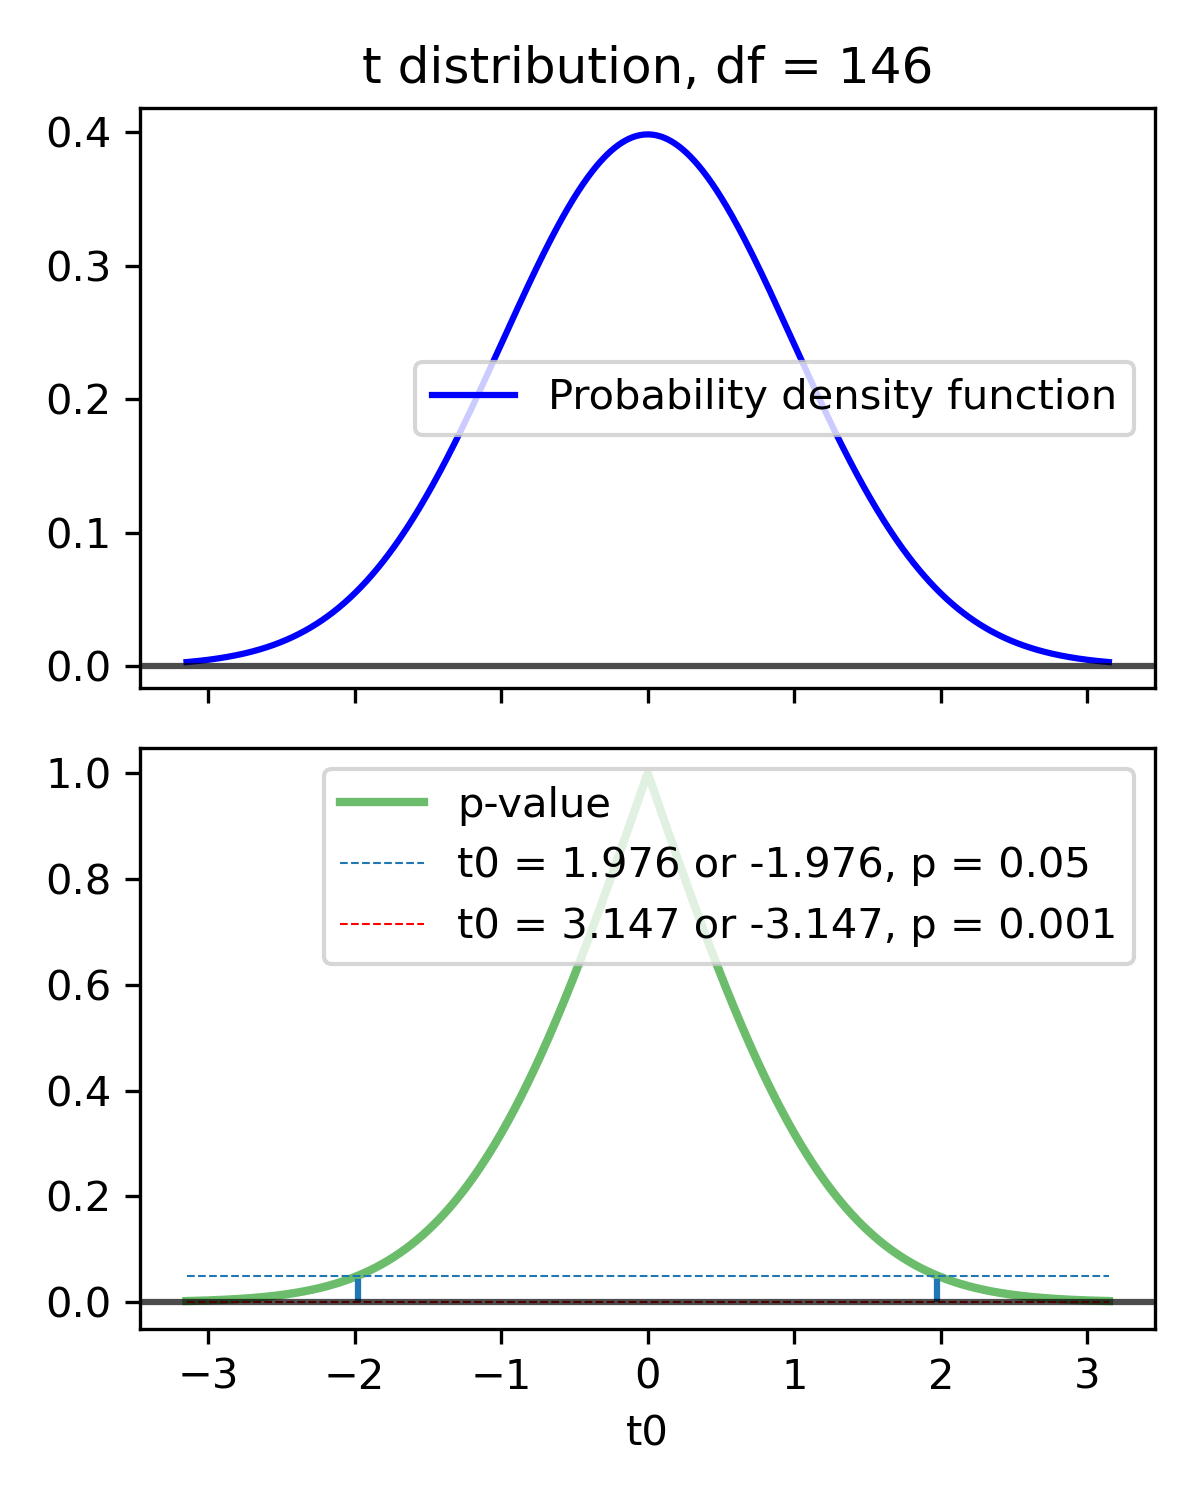
\includegraphics[width=0.5\textwidth]{figures/t-test.png}
	\caption{t-test of linear regression on \textit{diamonds} data set}
	\label{fig:t-test}
\end{figure}

Compare this to our four weights, we can determine that the first three weights have p-values significantly smaller than 0.05, indicating that it is very unlikely to get them by luck.
In contrast, the last weight $w_3$ has a p-value of 0.21, which is greater than 0.05, and thus not significant in terms of statistics.

What does this tell us?
The last weight, $w_3$, corresponds to the data attribute color scale. 
A P-value larger than 0.05 indicates this attribute may not be relevant. 
In other words, we can interpolate this as ``the value of a diamond is not affected by the color scale of that diamond''.
Therefore, we probably should not include this attribute in our model.
We will cover more advanced methods to properly deciding which attributes to include in our model in future posts. 

\section{Compare our code to existing packages with more examples}
Let's compare the results of our code to those of existing packages.
We choose \textit{sklearn.linear\_model.LinearRegression} in \textit{Python} and \textit{lm} in \textit{R} to compare.

\subsection{diamonds}
We already performed our liner regression code on \textit{diamonds} and we got the following result with $R^2 = 63.67\%$.
\begin{equation}
\text{diamond value} = 148.23+ 2.19 (\text{weight}) + 21.67(\text{clarity})-0.46(\text{color})
\end{equation}

Using \textit{sklearn}, we get the following result with $R^2 = 63.72\%$.
\begin{equation}
\text{diamond value} = 148.34 + 2.19 (\text{weight}) + 21.69(\text{clarity})-0.45(\text{color})
\end{equation}

Using lm in R, we get the following result with $R^2 = 63.73\%$.
\begin{equation}
\text{diamond value} = 148.33 + 2.19 (\text{weight}) + 21.69(\text{clarity})-0.45(\text{color})
\end{equation}

As plotted in Figure~\ref{fig:compare-diamonds}, majority of these three results overlapp with each other. 
\begin{figure}[htbp]
	\centering
	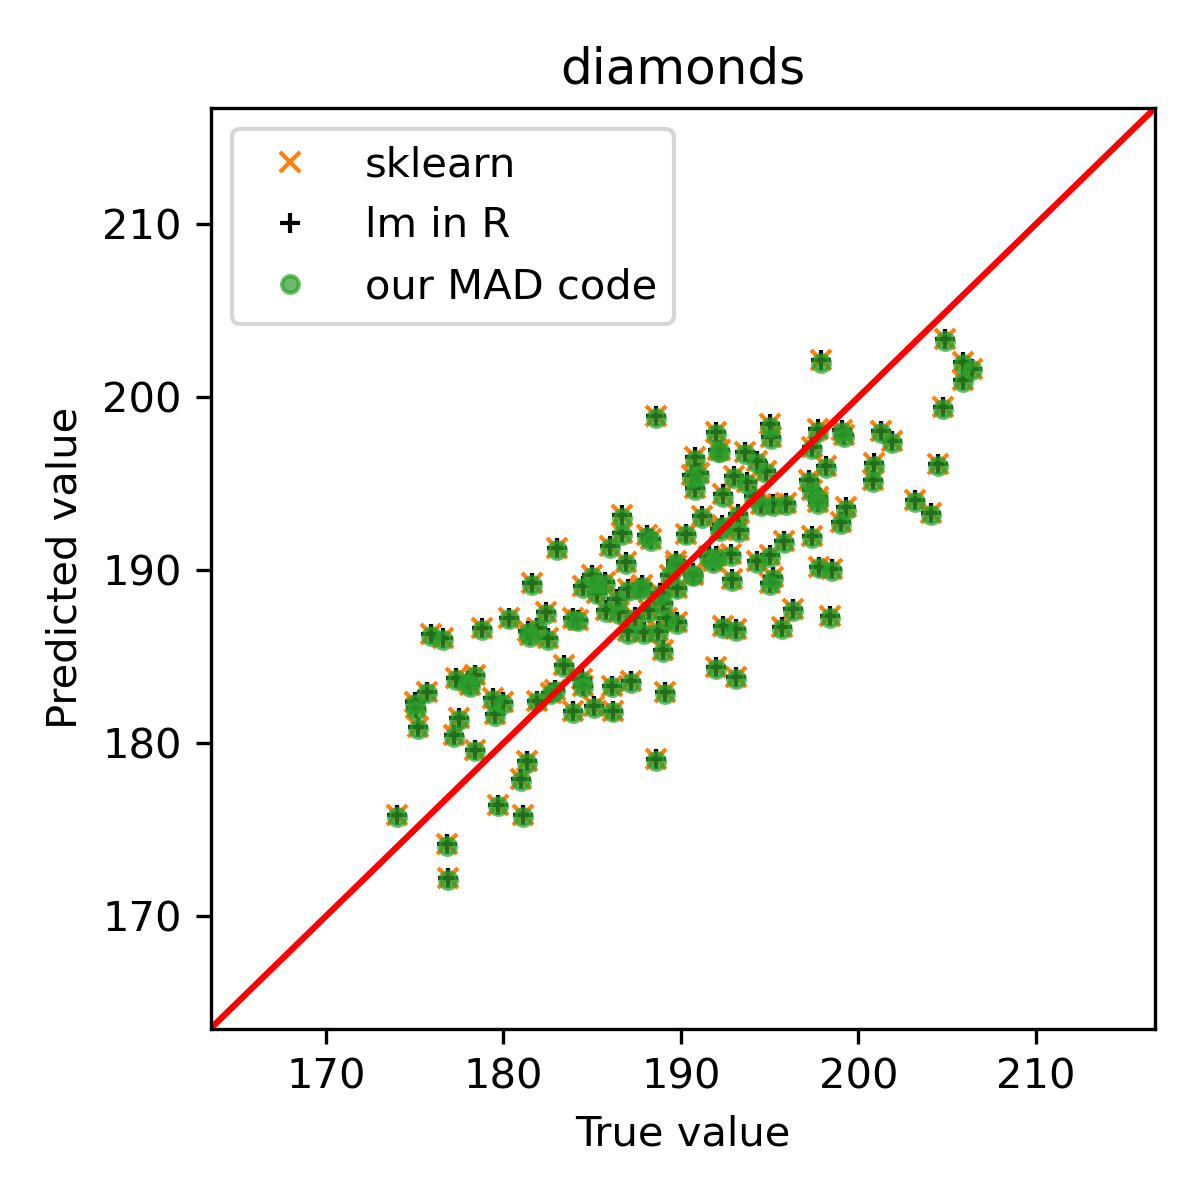
\includegraphics[width=0.65\textwidth]{figures/compare-diamonds.png}
	\caption{Compare our code to sklearn in Python and lm in R: \textit{diamonds} data set}
	\label{fig:compare-diamonds}
\end{figure}

\subsection{uscrime}
The data set \textit{uscrime} comes from \url{http://www.statsci.org/data/general/uscrime.html}.
This data set has 47 instances with 15 attributes such as unemployment rate, median family income, and so on. The outcome is crime rate.
\begin{figure}[htbp]
	\centering
	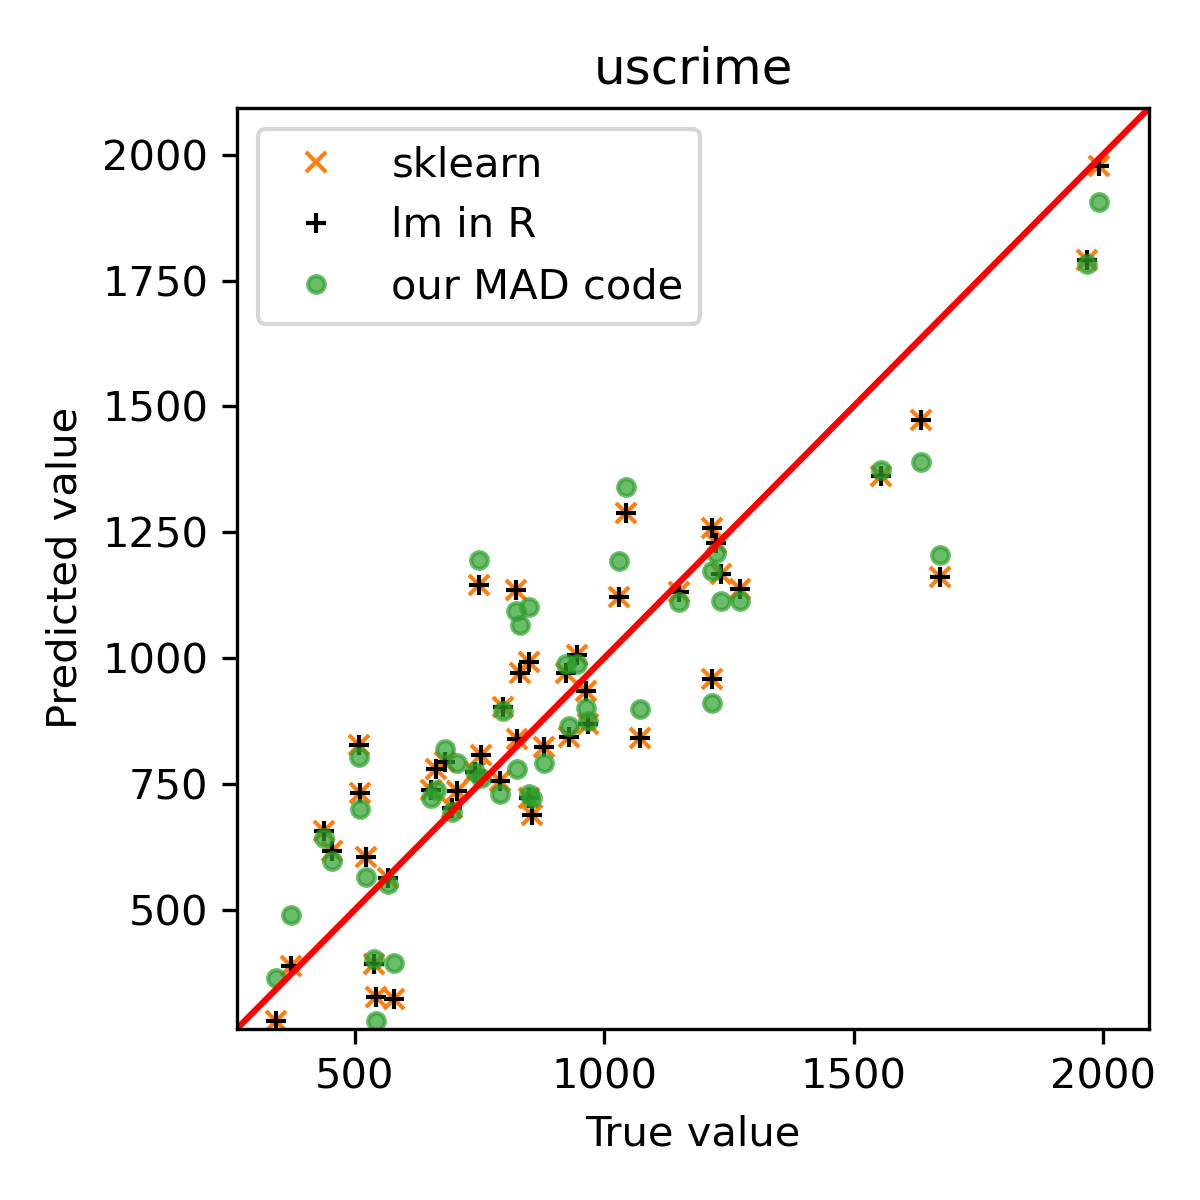
\includegraphics[width=0.65\textwidth]{figures/compare-uscrime.png}
	\caption{Compare our code to sklearn in Python and lm in R: \textit{uscrime} data set}
	\label{fig:compare-crime}
\end{figure}

\subsection{BostonHousing}
The data set \textit{BostonHousing} comes from \url{https://www.cs.toronto.edu/~delve/data/boston/bostonDetail.html}.
This data set has 506 instances with 13 attributes such as crime rate, property tax rate, and so on. The outcome is median house value.
\begin{figure}[htbp]
	\centering
	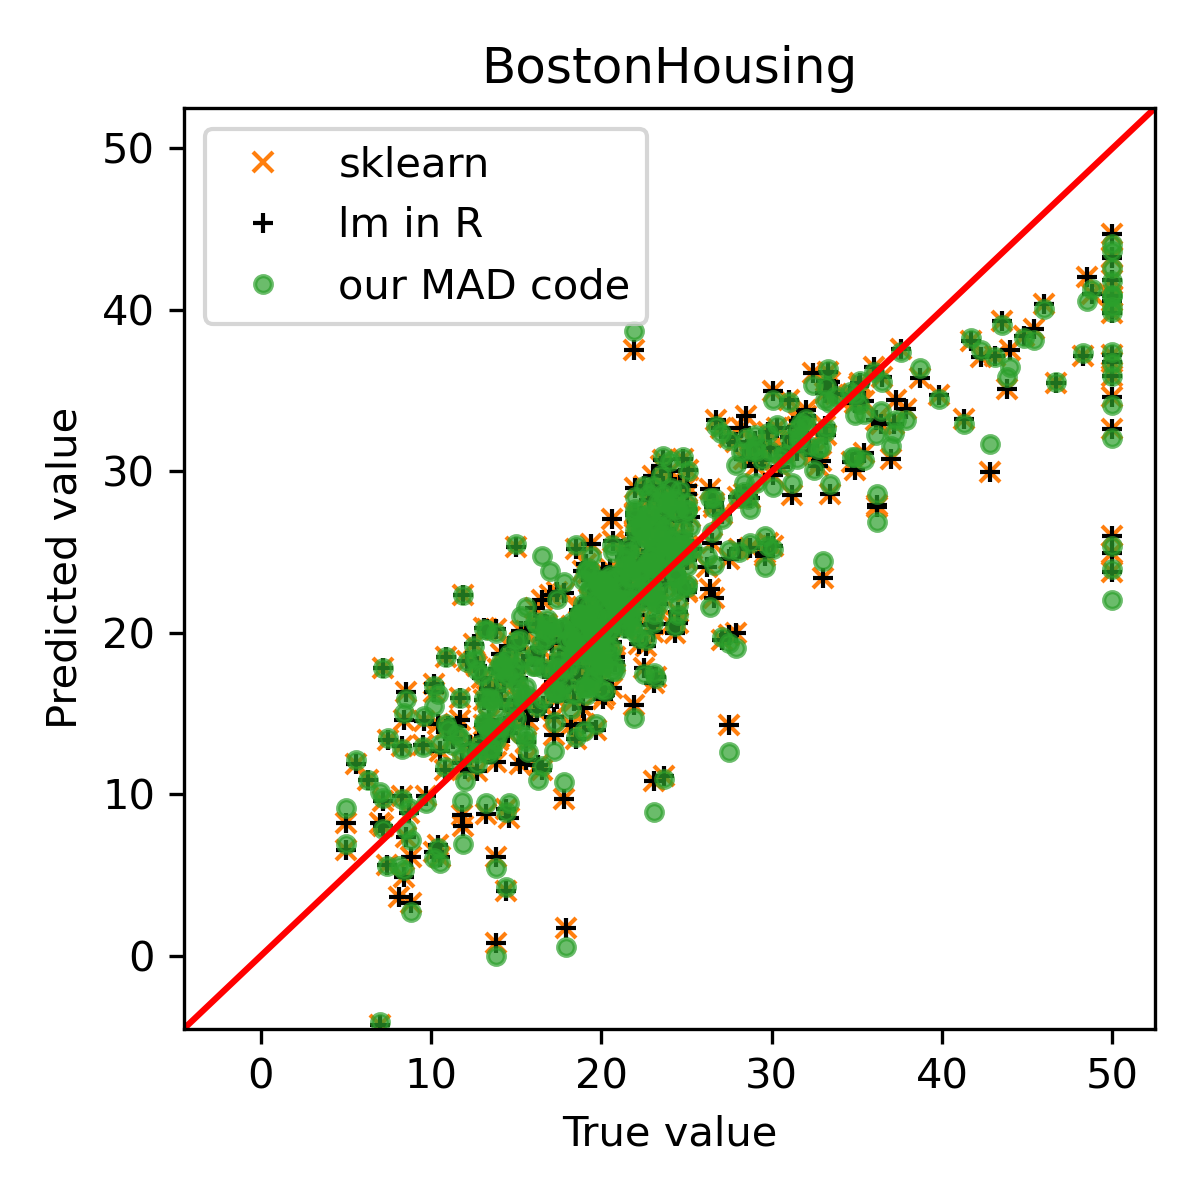
\includegraphics[width=0.65\textwidth]{figures/compare-BostonHousing.png}
	\caption{Compare our code to sklearn in Python and lm in R: \textit{uscrime} data set}
	\label{fig:compare-boston}
\end{figure}

\section{Summary}
We talked about basics of linear regression, then built a linear regression learner which achieved similar results as those of existing packages.




\end{document}